%for a more compact document, add the option openany to avoid
%starting all chapters on odd numbered pages
\documentclass[12pt]{cmuthesis}

% This is a template for a CMU thesis.  It is 18 pages without any content :-)
% The source for this is pulled from a variety of sources and people.
% Here's a partial list of people who may or may have not contributed:
%
%        bnoble   = Brian Noble
%        caruana  = Rich Caruana
%        colohan  = Chris Colohan
%        jab      = Justin Boyan
%        josullvn = Joseph O'Sullivan
%        jrs      = Jonathan Shewchuk
%        kosak    = Corey Kosak
%        mjz      = Matt Zekauskas (mattz@cs)
%        pdinda   = Peter Dinda
%        pfr      = Patrick Riley
%        dkoes = David Koes (me)

% My main contribution is putting everything into a single class files and small
% template since I prefer this to some complicated sprawling directory tree with
% makefiles.

% some useful packages
\usepackage{times}
\usepackage{fullpage}
\usepackage{graphicx}
\usepackage{amsmath}
\usepackage{amsfonts}
\usepackage{amssymb}
\usepackage{algorithm2e}
\usepackage{bbm}
\usepackage{multirow}
\usepackage{enumerate}
\usepackage[numbers,sort]{natbib}
\usepackage[backref,pageanchor=true,plainpages=false, pdfpagelabels, bookmarks,bookmarksnumbered,
%pdfborder=0 0 0,  %removes outlines around hyper links in online display
]{hyperref}
\usepackage{subfigure}

\DeclareMathOperator*{\argmin}{arg\,min}

% Approximately 1" margins, more space on binding side
%\usepackage[letterpaper,twoside,vscale=.8,hscale=.75,nomarginpar]{geometry}
%for general printing (not binding)
\usepackage[letterpaper,twoside,vscale=.8,hscale=.75,nomarginpar,hmarginratio=1:1]{geometry}

% Provides a draft mark at the top of the document. 
\draftstamp{\today}{DRAFT}

\begin {document} 
\frontmatter

%initialize page style, so contents come out right (see bot) -mjz
\pagestyle{empty}

\title{ {\it \huge Thesis Proposal}\\
{\bf Knowledge-aware Natural Language Understanding}}
\author{Pradeep Dasigi}
\date{}
\Year{2017}
\trnumber{}

\committee{
Eduard Hovy (Chair) \\
Chris Dyer \\
William Cohen \\
Luke Zettlemoyer
}

\support{}
\disclaimer{}

% copyright notice generated automatically from Year and author.
% permission added if \permission{} given.

\keywords{natural language understanding, knowledge, neural networks, end-to-end models, semantic parsing, question answering}

\maketitle

% TODO: Uncomment this for the dissertation
% \begin{dedication}
% 
% \end{dedication}

\pagestyle{plain} % for toc, was empty

%% Obviously, it's probably a good idea to break the various sections of your thesis
%% into different files and input them into this file...

\begin{abstract}
Natural Language Understanding (NLU) systems
process human generated text (or speech) at a deep semantic level in a way that is useful for downstream applications such as
question answering, textual entailment or summarization. In this thesis, we examine the role of 
knowledge in NLU, and build systems that effectively encode and reason over knowledge.
We identify two kinds of knowledge, and make the following distinction between them: \textbf{implicit knowledge} is that which
is missing in the input utterances, but necessary for understanding them, and \textbf{explicit knowledge} is the additional context that
NLU systems need to reason over, for complete comprehension. A generic NLU pipeline typically involves two main components. 
The first is \textbf{encoding}, where words (or other basic linguistic units) within the inputs are composed to compute encoded representations, 
which are then used as features in the second component, \textbf{prediction}, to produce the desired output. We describe several NLU systems
that follow this pipeline, but with encoders that also encode implicit knowledge, or predictors that effectively reason over explicit knowledge.

The first part of the thesis deals with implicit or background knowledge. While distributional methods for encoding inputs have been
successfully used to represent meaning of words in the context of other words in the input,
and thus learn complex functions of their distributional properties, there are other aspects of semantics that are out of their reach. These aspects are related to
commonsense or real world information which is part of shared human knowledge but is not explicitly present in the input. We address this limitation
using two methods that rely on external resources. The first is by modeling the selectional restrictions verbs place on their
semantic role fillers. We use this model to encode events, and show that these event representations are useful in detecting newswire anomalies.
Our second approach towards augmenting distributional methods is using external knowledge bases like WordNet. We compute
ontology-grounded token-level representations of words and show that these representations are useful in predicting prepositional phrase attachments and textual entailment.

The second part of the thesis focuses on reasoning over explicit knowledge. Many machine comprehension tasks require interpreting input utterances in context of other explicit structured
or unstructured information. For structured contexts, we first describe a type constrained neural semantic parsing framework for answering questions
given semi-structured tables as the context. With simple entity linking and context-graph embedding methods, we achieve state of the art performance on the \textsc{WikiTableQuestions} dataset.
Proposed work in this area includes improved entity linking, and application of this framework to answering questions in other domains. For unstructured contexts, we propose to investigate
the role of retrieval methods for obtaining contexts in question answering using neural network models with explicit memory components,
and build models that can adaptively reason and learn to retrieve relevant context given a question.

\end{abstract}

% TODO: Uncomment this for the dissertation
% \begin{acknowledgments}
% 
% \end{acknowledgments}



\tableofcontents
\listoffigures
\listoftables

\mainmatter

%% Double space document for easy review:
%\renewcommand{\baselinestretch}{1.66}\normalsize

% The other requirements Catherine has:
%
%  - avoid large margins.  She wants the thesis to use fewer pages, 
%    especially if it requires colour printing.
%
%  - The thesis should be formatted for double-sided printing.  This
%    means that all chapters, acknowledgements, table of contents, etc.
%    should start on odd numbered (right facing) pages.
%
%  - You need to use the department standard tech report title page.  I
%    have tried to ensure that the title page here conforms to this
%    standard.
%
%  - Use a nice serif font, such as Times Roman.  Sans serif looks bad.
%
% Other than that, just make it look good...


\chapter{Introduction}
\label{chapter:introduction}
\section{Natural Language Understanding}
A Natural Language Understanding (NLU) system processes human generated text (or speech) at a deep semantic level and encodes the meaning
of the processed inputs, such that it can perform well at the task for which it is designed. NLU is thus an umbrella term that includes several
tasks, that can be defined in terms of their end goals. For example, Question Answering (QA), an NLU task, refers to answering questions about a span of text,
or other structured knowledge representations like knowledge bases or even images.
QA systems are required to encode the meaning of the provided inputs such that the relevant bits of information can be retrieved to answer questions.
Recognizing Textual Entailment (RTE), another NLU task, refers to the problem of identifying whether the truth value of some text provided as a hypothesis follows from that of another 
text provided as a premise, and it is usually done by extracting relevant features from the hypothesis and the premise to see if there is enough
overlap between them in the right direction. Another example of an NLU task is Sentiment Analysis, which is automatically categorizing the opinions expressed in the input
utterances towards specific targets, which involves extracting appropriate affective states and subjective information, such that a sentiment classifier
can be built using that information as features. All these tasks require encoding the semantics of the input in a way that is
at least good enough to perform well at the given task, with the inherent assumption that an improvement in the task performance correlates with an improvement in the
quality of the semantic representation, or in other words, the understanding capability of the computational system.

In each of the examples above, it can be noticed that there are two common components: an \textbf{encoder} and a \textbf{predictor}. The encoder
extracts task-relevant features from the input, and the predictor performs the appropriate computation on top of the features given by the encoder
to produce the desired result. A generic NLU system can thus be succinctly described using the
following two equations.
\begin{align}
 \mathbf{e} &= \mathtt{encode}(\mathbf{I}) \label{eq:generic_encoding}\\
 \mathbf{o} &= \mathtt{predict}(\mathbf{e}) \label{eq:generic_prediction}
\end{align}
where $\mathbf{I}$ is the set of textual inputs to the NLU system. 
For example, $\mathbf{I}$  are single sentences in Sentiment Analysis and pairs of sentences in RTE. $\textbf{e}$ are intermediate 
encoded semantic representations of the inputs (which may or may not be task specific), and $\mathbf{o}$ are the final task specific predictions. For example, in Sentiment Analysis or RTE, 
$\mathbf{o}$ are categorical labels indicating the sentiment or entailment respectively, and in the case of Semantic Parsing, they are structured outputs or parses.

In older feature-rich methods for NLU, 
Equation~\ref{eq:generic_encoding} is a mapping of the inputs to a hand designed feature space, typically containing patterns over word classes based on
part-of-speech \citep{corley2005measuring} or Wordnet synsets \citep{moldovan2001logic} shallow linguistic features like dependencies \citep{bos2005recognising}
named entity information \cite{tatu2005semantic}, or other features depending on the task. The choice of features was left to the discretion of the ML-practitioners
designing the NLU systems. In such systems, the modeling emphasis was more on the prediction component, and the encoding component did not involve any learning. 
More recent systems \citep[among many others]{bahdanau:14,weston2014memory,hermann2015teaching,Xiong2016DynamicMN,bowman2016fast,yang:16} 
use representation learning or deep learning techniques to also learn the parameters of the
$\mathtt{encode}$ function, and typically this is done jointly with learning the parameters of the $\mathtt{predict}$ function, to ensure task-relevancy.

\section{Knowledge}
\label{sec:intro_external_knowledge}
A computational system that seeks to understand human utterances, cannot do so given the utterances alone. This is because, the utterances themselves
do not contain all the information needed to comprehend them. The missing information is either part of the background knowledge about the world humans
inherently possess, or the surrounding context in which the utterance is spoken or written. NLU systems thus need to access this knowledge to comprehend
human languages.

In this thesis, we distinguish between background or implicit knowledge, and contextual or explicit knowledge. We now describe them in the context of NLU.

\subsection{Background Knowledge}
An issue with the formulation of the problem in Equation~\ref{eq:generic_encoding} is that it is missing a key input: \textbf{background knowledge}. 
Since human language is aimed at other humans who share 
the same background knowledge, a lot of information is often not explicitly stated
for the sake of brevity. The implicit knowledge required to understand language varies 
from simple commonsense in the case of basic conversations, to complex principles that link 
concepts in more esoteric communications.

The notion of implicit knowledge can be illustrated using the following example. Consider the
events described by the following two sentences:

\begin{itemize}
 \item[] \textit{Cops shoot a man.}
 \item[] \textit{Man shoots a dog.}
 \item[] \textit{Dog shoots a man.}
\end{itemize}

Clearly, one would find the third sentence more unusual compared to the first and the second, the reason being that
a \emph{dog} performing a \emph{shooting} action does not agree with our knowledge about the general state
of affairs. While this information is not clearly written down anywhere, humans know it implicitly. An NLU
system that is designed to differentiate between these sentences should be provided with the information
that \emph{dog} in the role of the agent for \emph{shooting} is unlikely, while it can be the patient for
\emph{shooting}, and \emph{man} fits equally well as agent and patient for \emph{shooting}. The notion that
some combinations of actions and their arguments are more semantically likely than others is referred to as
Selectional Preference \citep{wilks1973preference}, and we describe that in greater detail in Chapter~\ref{chapter:nem}.

Consider another example of the need for encoding commonsense information, that of solving the 
textual entailment problem given the following premise, and candidate hypothesis:
\begin{itemize}
 \item[] \textbf{Premise:} \textit{Children and parents are splashing water at the pool.}
 \item[] \textbf{Hypothesis} \textit{Families are playing outside.}
\end{itemize}
The knowledge a human uses to correctly predict that the hypothesis can be inferred from the 
premise is that \textit{children and parents} typically form \textit{families}, \textit{splashing water} 
is a kind of \textit{playing}, and a \textit{pool} is expected to be \textit{outside}. An entailment model trained on texts like the
ones shown above, with just the sentences as inputs, will not have access to the background knowledge that humans possess.
% TODO: Give a PPA example here?
Such a model will at best memorize co-occurrence patterns in the input words. Using pre-trained vectors to represent input words provides additional
knowledge to the model in the form of co-occurrence statistics obtained from large corpora. However, it is unclear whether distributional
information at the word level alone can substitute for the kind of knowledge described above.
Fortunately, background knowledge of this kind is encoded to some extent in machine readable
ontologies and knowledge bases.

In this thesis, we will show how such background knowledge can be encoded either by leveraging Selectional Preferences
or by incorporating external knowledge sources, and used in conjunction with distributional models to obtain better input representations
for NLU systems.

\subsection{Contextual Knowledge}
A second issue with the generic NLU formulation, particularly with Equation~\ref{eq:generic_prediction}, is that it does not account for the context
in which the input utterance occurs. Typically, context includes the circumstances that form the setting for the input utterances to be fully understood,
and hence it significantly contributes to the meaning of the inputs. In this thesis, we will refer to this additional information as \textbf{contextual knowledge}.
Unlike background knowledge, this is not implicit in the
text being read. However, reasoning in the presence of contextual knowledge still poses significant challenges. An automated reading comprehension system that
reasons over this additional information is expected to effectively do the following: encode the context in such a way that the bits of information relevant to the input
utterances can be aligned to the input; encode the inputs in such a way that they can be executed against the encoded context to produce the desired output. Approaches
for encoding inputs and contexts, and linking them depend on the nature of the contextual information.

%TODO: The following paragraph needs to be improved.
In the case of structured contexts, such as knowledge graphs, linking contexts
to inputs is referred to as \emph{entity linking}, and encoding inputs is a \emph{Semantic Parsing} problem, where the natural language utterances are translated into
logical forms that can be executed against the knowledge graph to produce the desired output.
% TODO: Give examples of semantic parsing papers.
When the contexts are unstructured, the problem boils down to encoding the context in a way to facilitate extracting input-specific information from it. This is usually
referred to as \emph{Information Extraction}.
Examples include \cite{hill2015goldilocks,richardson2013mctest,penas2013qa4mre,breck2001looking}.
In this thesis, we focus on both structured and unstructured contexts.

Figure~\ref{fig:wikitables_example} shows a question taken from the Wikitables dataset \citep{pasupat2015compositional}, and an associated table from a Wikipedia article,
which provides the necessary context to answer it. This an example of a QA task where the context is (semi) structured. As it can be seen from the example, answering this
question requires doing multi-step reasoning over the table.
\begin{figure}
\begin{center}
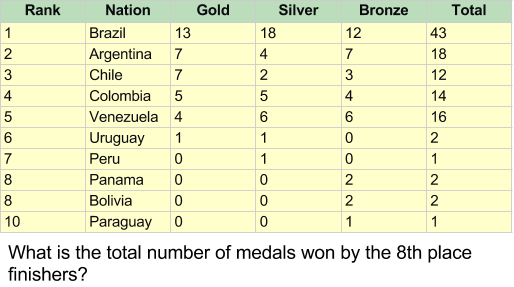
\includegraphics[width=4in]{figures/wikitables_example.png}
\caption{Example of a task requiring reasoning over semi-structured context}
\label{fig:wikitables_example}
\end{center}
\end{figure}

Figure~\ref{fig:babi_example} shows an example where the context is unstructured. This is from the bAbI dataset \citep{weston2015towards}, which is a collection of artificially generated toy tasks.
The first six sentences in the example
form the context, and the final line is a question followed by the answer and pointers to the relevant sentences in the context. A QA system is expected to learn to find the appropriate context
given the question and answer it correctly.
\begin{figure}
\begin{center}
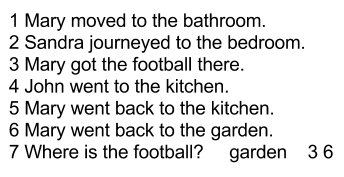
\includegraphics[width=3in]{figures/bAbI_example.png}
\caption{Example of an artificial task requiring reasoning over context, part of the bAbI dataset}
\label{fig:babi_example}
\end{center}
\end{figure}

Figure~\ref{fig:science_qa_example} shows a relatively more difficult QA example from Aristo science question answering dataset \citep{clark2015elementary}. Simple techniques such as measuring lexical overlap do not
work well for this task because all four options have significant overlap with the sentences in context. As we show in Chapter~\ref{chapter:memnet_qa}, this task requires modeling complex entailment to be able to match the information present in the context with that in the question and
option pairs.
\begin{figure}
\begin{center}
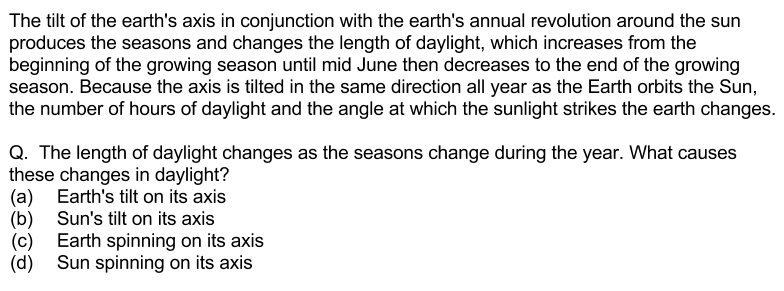
\includegraphics[width=6in]{figures/science_qa_example.png}
\caption{Snippet from a science textbook followed by a question}
\label{fig:science_qa_example}
\end{center}
\end{figure}


\section{Knowledge-Aware NLU}
Given that knowledge, both implicit and explicit, plays an important role in several real-world language understanding tasks, we need to reconsider
our definition of the generic NLU pipeline.
Without background knowledge, the encoding of inputs will be incomplete, and the NLU systems might not generalize beyond the specific patterns 
seen in the training data to unseen test cases. Without contextual knowledge, and an effective method to link encoded inputs to contexts, the NLU
systems will simply not have sufficient information to produce the desired results. We thus modify our NLU equations as follows.
\begin{align}
 \mathbf{e} &= \mathtt{encode\_with\_background}(\mathbf{I}, \mathbf{K}_e) \label{eq:encoding_with_knowledge}\\
 \mathbf{e}_{K_p} &= \mathtt{encode\_context}(\mathbf{K}_p) \\ \label{eq:knowledge_encoding}
 \mathbf{o} &= \mathtt{predict\_with\_context}(\mathbf{e}, \mathbf{e}_{K_p}) \label{eq:prediction_with_knowledge}
\end{align}
where $\mathbf{K}_e$ and $\mathbf{K}_p$ represent the knowledge required for encoding and prediction respectively. They
come from different sources and augment the inputs in different ways.

Obtaining relevant background or contextual
knowledge can be challenging as well, depending on the task being solved. In this thesis, we do not put a lot of emphasis on these
problems, except in Chapter~\ref{chapter:memnet_qa}, where we focus on context retrieval. In the remaining chapters, we will focus on tasks
and datasets where obtaining appropriate knowledge is easy.

\paragraph{Better encoding with background knowledge}
$\mathbf{K}_e$ is additional knowledge used to better compose the units in input text. Particularly, this allows for
obtaining input encoding that respects the selectional restrictions of the units being composed.
Examples of $\mathbf{K}_e$ include hypernym trees from WordNet for
incorporating sense and generalization information about concepts while composing sentences and subgraph features from Freebase to encode relations
between entities seen in the input text. \cite{moldovan2001logic} and \cite{krymolowski1998incorporating} are examples of a feature-rich systems that encoded input sentences in the 
context of external knowledge. Both systems used WordNet features and other related information about the semantic classes of the words in the input in NLU tasks. While \cite{krymolowski1998incorporating} 
built a system based on SNoW \citep{CCRR99} for predicting Prepositional Phrase Attachment, \cite{moldovan2001logic} built a Question answering system. In Chapter~\ref{chapter:ontolstm} we describe
a representation-learning application of knowledge-aware encoding where we show the advantages of incorporating WordNet information in recurrent neural networks for encoding sentences. In Chapter~\ref{chapter:nem},
we leverage selectional preferences in SRL structures to build an NLU system that understands events in the newswire domain.

\paragraph{Reasoning with contextual knowledge}
$\textbf{K}_p$ inputs allow the prediction step to reason in the context of additional knowledge. $\textbf{K}_p$ can either be structured or unstructured. In cases where it is structured,
reasoning with it involves producing structured representations of inputs that can be executed against it, and the task becomes Semantic Parsing, which was dealt with using
both traditional \citep[among others]{Zelle1996LearningTP,Zettlemoyer2005LearningTM,zettlemoyer2007online} and neural network based methods
\citep{Dong2016LanguageTL,Andreas2016LearningTC,Liang2016NeuralSM,Neelakantan2016LearningAN}. We build on top of this work on Semantic Parsing, and describe a type driven neural semantic 
parsing framework in Chapter~\ref{chapter:nnsp}.

Machine reading comprehension also involves reasoning over contexts, but unstructured ones. This task typically involves encoding some context given as a paragraph and using it to
produce an answer from an encoded question. Examples of task targeted datasets built to evaluate that capability include MCTest \citep{Richardson2013MCTestAC},
CNN/Daily Mail dataset \citep{hermann2015teaching}, SQuAD \citep{Rajpurkar2016SQuAD10} and TriviQA \citep{Joshi2017TriviaQAAL}, among others.
Systems built for these tasks including attentive readers \citep{hermann2015teaching}, variants of memory networks \citep{weston2014memory,Sukhbaatar2015EndToEndMN,Xiong2016DynamicMN}
and the more recent Bidirectional Attention Flow \citep{Seo2016BidirectionalAF} can be viewed as different instantiations
of the $\mathtt{predict\_with\_context}$ function, where $\textbf{K}_p$ is some background text that needs to be understood to answer a question about it. 
In Chapter~\ref{chapter:memnet_qa}, we describe a generic formulation of the problem.

\section{Challenges}
%TODO: Challenges with using selectional preferences

Adding external knowledge inputs to NLU systems is not straightforward.  Firstly, while linking text being read to some structured background knowledge
in a KB, an automated system faces ambiguity. For example, with lexical ontologies like WordNet, 
we get useful type hierarchies like \textit{parent is-a ancestor is-a person} and \textit{pool is-a body-of-water} 
and so on, but one has to deal with sense ambiguity: \textit{pool} can also be a game. Moreover, the fact that the two sources of semantic information are fundamentally different 
makes this challenging. While distributional approaches encode meaning in a
continuous and an abstract fashion, meaning in KBs is symbolic and discrete. Chapter~\ref{chapter:ontolstm} is dedicated to learning 
distributions over the discrete concepts of the KB conditioned on the context, to deal with exceptions in language.

%TODO: Chalenges in Semantic Parsing

When reasoning in the presence of context, finding the 
relevant parts of the provided information given the text being processed is a challenge. 
The goal of this thesis is to find the limitations of various knowledge sources -- structured and unstructured -- and use this information 
to build hybrid NLU systems that can successfully incorporate real world knowledge in deep learning models. We now describe how this thesis is organized.

\section{Thesis Outline}
\begin{figure}
\begin{center}
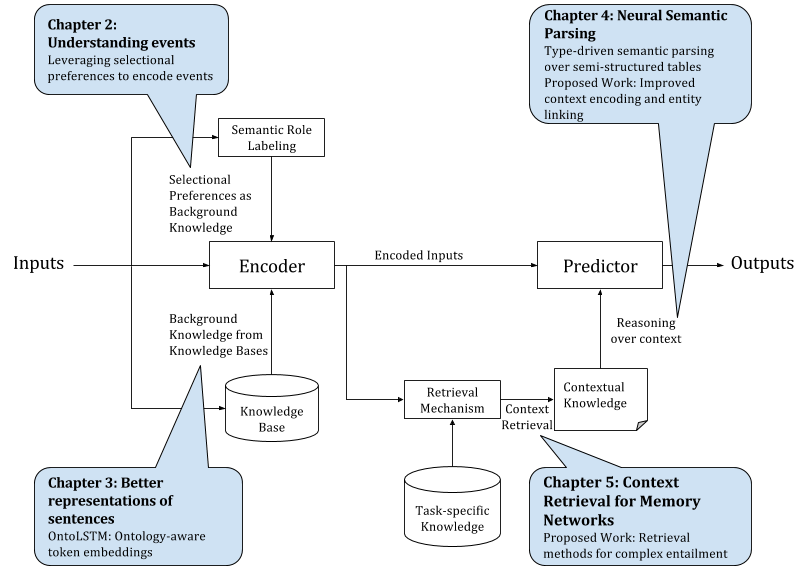
\includegraphics[width=6.5in]{figures/thesis_overview.png}
\caption{Generic NLU pipeline and thesis overview}
\label{fig:thesis_overview}
\end{center}
\end{figure}
Figure~\ref{fig:thesis_overview} shows the generic pipeline described so far, along with the breakdown of the chapters related to each component
of the pipeline.

In Chapter~\ref{chapter:nem} we encode events as predicate argument structures derived from a semantic role labeler.
In this chapter, we rely on selectional preferences between verbs and their semantic role fillers as the background
knowledge, and show how they are useful in predicting anomalous events.
Our event encoder, Neural Event Model (NEM) captures semantics deeper than surface fluency. We describe an annotation effort that
resulted in newswire headlines manually labeled with the degree of surprise associated with them and show that NEM outperforms
a baseline LSTM model that encodes sentences at anomaly detection. 

In Chapter~\ref{chapter:ontolstm}, we describe a method to incorporate implicit knowledge
from WordNet, towards obtaining better sentence representations. Our model looks at WordNet synsets,
and at the hypernym hierarchies of the words being processed so that the 
encoder is aware of their different senses, and the corresponding type information.
The ontology aware LSTM (OntoLSTM) learns to attend to the appropriate sense,
and the relevant type 
(either the most specific concept or a generalization by choosing a hypernym of
the word), conditioned on the context and the end-objective. We show that the sentence representations 
produced by OntoLSTM are better than those produced by LSTMs when used with identical prediction 
components for predicting textual entailment and preposition phrase attachment. We also visualize the attention scores assigned to the hypernyms 
of words in the input sentences and show that OntoLSTM is indeed learning useful generalizations of words
that help the learned representations perform better at the end task.

Chapter~\ref{chapter:nnsp} deals with reasoning over semi-structured contexts. We describe a type-driven
neural semantic parser aimed at answering compositional questions on Wikipedia tables. It is an encoder-decoder model that generates
well-typed logical forms that can be executed against graph representations of the tables in context. The parser also includes entity embedding
and linking modules that are trained jointly using QA supervision. This parser achieves state-of-the art result on \textsc{WikiTableQuestions} dataset.
Proposed work includes improving the entity linking module, and applying this parser to QA in other domains.

The focus of Chapter~\ref{chapter:memnet_qa} is on context retrieval methods for neural network models with explicit memory components.
We start by describing a generalized deep learning architecture for reasoning over unstructured contexts. The pipeline follows the generic
specification in Section~\ref{sec:intro_external_knowledge} and has configurable components
for encoding and prediction. We identify that the memory network models in \cite{weston2014memory,Sukhbaatar2015EndToEndMN,Xiong2016DynamicMN}
and the attentive reader model from \cite{hermann2015teaching} are specific instantiations of our generic knowledge guided reasoning model.
Unlike prior work that evaluated these models on tasks where the contexts are limited and well-defined, we deal with tasks that require
retrieving relevant context from large corpora. Our preliminary experiments show that the choice of retrieval methods greatly affect the
final QA results. Based on this insight, we propose to build models where retrieval is tightly integrated in the QA pipeline.

% Finally, in Chapter~\ref{chapter:transfer_learning}, we propose to investigate the transferability of the representations learned for one NLU task to other tasks.
% Transfer Learning in neural networks has been well-studied in vision related tasks, and it has been established that the features learned for one task can be
% used to improve the performance of similar architectures in other tasks. Within the scope of NLU, this is a feasible investigation given that similarity
% among the neural network architectures used for various tasks. It is an important investigation because not all tasks come with lots of training data, owing to factors
% such as difficulty in getting reliable annotations and subjectivity. Moreover, with the current trend of increasing model complexity to perform better at any given task,
% it is becoming increasingly important to ensure that the models do not overfit any given dataset.
\part{Encoding Implicit Knowledge}
\chapter{Leveraging Selectional Preferences for Event Understanding}
\label{chapter:nem}
\section{Introduction}
In this chapter, we describe a system that models implicit knowledge by exploiting the structure
in inputs. Our approach relies on the co-occurrence of fillers of slots given by the structure to
capture this knowledge. This notion was referred to as Selectional Preference \cite{wilks1973preference}
in earlier literature (see Section~\ref{sec:nem_background} for more information). While this notion was earlier
restricted to verbs and their arguments in dependency structures, we hypothesize that it extends to
other kinds of structures as well, and consequently, it can be used for modeling appropriate implicit semantic knowledge.

This chapter shows one instantiation of implicit knowledge, and we select the appropriate structures to model selectional
preferences in. The task presented here is that of differentiating between normal news headlines and strange or weird ones,
and the implicit knowledge required for this task is fundamental to understanding events. Hence, we obtain the structured
representations of the input utterances from a Semantic Role Labeler, a tool which identifies the eventive predicate in a given
input sentence, and its corresponding role fillers.

\section{Understanding Events}
Events are fundamental linguistic elements in human speech. Thus understanding 
events is a fundamental prerequisite for deeper semantic 
analysis of language, and any computational system of human language should
have a model of events. One can view an event as an occurrence of a certain 
action caused
by an agent, affecting a patient at a certain time and place and so on. It is 
the combination of the entities
filling the said roles that define an event. Furthermore, certain combinations 
of these role fillers
agree with the general state of the world, and others do not. For example, 
consider the events described by the following
sentences.
\begin{itemize}
 \item[] \textit{Man recovering after being bitten by his dog.}
 \item[] \textit{Man recovering after being shot by cops.}
\end{itemize}
The \textit{agent} of the \textit{biting} action is \textit{dog} in the first 
sentence, and that of the \textit{shooting}
action in the second sentence is \textit{cops}. The patient in both sentences is 
\textit{man}.
Both combinations of role-fillers result in events that agree with most people's 
world view. That is not the case with
the event in the following sentence.
\begin{itemize}
 \item[] \textit{Man recovering after being shot by his dog.}
\end{itemize}
This combination does not agree with our expectations about the general state of 
affairs, and consequently one
might find this event strange. While all three sentences above are equally
valid syntactically, it 
is our knowledge about the role fillers 
---both individually and specifically in combination---  
that enables us to 
differentiate between normal and anomalous events.  Hence we hypothesize that
\emph{anomaly is a result of unexpected or 
unusual combination of semantic role fillers}.

In this chapter, we introduce the problem of automatic anomalous event
detection and propose a novel event model that can learn to differentiate
between normal
and anomalous events. We generally define anomalous events as those that are
unusual compared
to the general state of affairs and might invoke surprise when reported. An 
automatic
anomaly detection algorithm has to encode
the goodness of semantic role filler coherence.  This is a hard problem since
determining what a good combination of role fillers is 
requires deep semantic and pragmatic knowledge.  
Moreover, manual judgment of anomaly itself may be difficult and people often
may not agree with each other in this
regard.  We describe the difficulty in human judgment in greater detail in
Section~\ref{sec:nem_annot}.  
Automatic detection of anomaly requires encoding complex information, which
poses the challenge of sparsity
due to the discrete representations of meaning, that are words.  These problems
range from polysemy and synonymy at the 
lexical semantic level to entity and event coreference at the discourse level.

We define an event as the pair $(V, \textbf{A})$, where $V$
is the predicate or a semantic verb\footnote{By semantic verb, we mean an action 
word whose
syntactic category is not necessarily a verb.  
For example, in \textit{Terrorist attacks on the World Trade Center..},
\textit{attacks} is not a verb but is still an 
action word.}, and $\textbf{A}$ is the set of its semantic arguments like agent,
patient, time, location, so on. Our aim
is to obtain a vector representation of the event that is composed from
representations of individual words, while explicitly guided by the semantic
role structure. This representation can be understood as an embedding of the
event in an event space. 

\section{Related Work} \label{sec:nem_background}
Selectional preference, a notion introduced by \cite{wilks1973preference}, 
refers to the paradigm of modeling semantics of
natural language in terms of the restrictions a verb places on its arguments. 
For example, the knowledge required to identify
one of the following sentences as meaningless can be encoded as preferences (or 
restrictions) of the verb.
\begin{itemize}
 \item[] \textit{Man eats pasta.}
 \item[] \textit{Poetry eats computers.}
\end{itemize}
The restrictions include \textit{eat} requiring its subject to be animate, its 
object to be edible, and so on. Though the
notion was originally proposed for a verb and its dependents in the context of 
dependency grammars, it is equally applicable to
other kinds of semantic relations. In this work,
we use this idea in the context of verbs and their semantic role fillers.

The idea is that identifying the right sense of the word can be guided by the 
preferences of the other words it is related to.  \cite{resnik1997selectional}
illustrates this through the example of disambiguating the sense of the word 
\textit{letter} in the phrase \textit{write a letter}.
While \textit{letter} has multiple senses, as an object, the verb \textit{write} 
``prefers'' the sense closer to \textit{reading matter} more than others.
At the phrasal level, selectional preferences are useful in encoding complex 
phenomena like metaphor.  Metaphorical usage of words usually involves violating 
selectional restrictions.
For example the phrase \textit{kill an idea} is a metaphor, because 
\textit{kill} does not usually take abstract concepts as objects.  The phrase 
itself is common and
one can easily attribute a metaphorical sense to the verb kill and resolve the 
violation.  \cite{wilks2007making}, \cite{wilks2007preferential}, 
\cite{krishnakumaran2007hunting},
\cite{shutova2013statistical}, among others discuss the selectional preference 
view of metaphor identification.
Automatic acquisition of selectional preferences from text is a well studied 
problem.  \cite{resnik1996selectional} proposed the first broad coverage 
computational model of selectional preferences.  The approach is based on using 
WordNet's hierarchy to generalize across words.
It measures selectional association strength of an triple $(v, r, c)$ with verb 
$v$, relation $r$ and an argument class $c$ as the Kullback-Leibler divergence 
between the the distributions $P(c|v, r)$  $c$
and $P(c|r)$ normalized over all classes of arguments that occur with the $(v, 
r)$ pair.  \cite{abe1996learning} also use WordNet, and model selectional 
preferences by minimizing the length tree cut through
the noun hierarchy.  \cite{ciaramita2000explaining} encode the hierarchy as a 
Bayesian network and learn selectional preferences using probabilistic graphical 
methods.
\cite{rooth1999inducing} take a distributional approach, and use latent variable 
models to induce classes of noun-verb pairs, and thus learn their preferences.  
Methods by \cite{erk2007simple,erk2010flexible}
are also distributional, and have been described earlier in this paper.  
\cite{seaghdha2010latent} proposed the use of Latent Dirichlet Allocation (LDA), 
to model preferences as topics.  \cite{van2009non} used
non-negative tensor factorization, and modeled subject-verb-object triples as a 
three-way tensor.  The tensor is populated with co-occurrence frequencies, and 
the selectional preferences are measured from decomposed
representations of the three words in the triple. \cite{van2014neural} trains 
neural networks to score felicitous triples higher than infelicitous ones.

\cite{erk2010flexible} also model selectional preferences using vector spaces.  
They measure the 
goodness of the fit of a noun with a verb in terms of the similarity between the 
vector of the noun and 
some ``exemplar'' nouns taken by the verb in the same argument role.  
\cite{baroni2010distributional} 
also measure selectional preference similarly, but instead of exemplar nouns, 
they calculate a 
prototype vector for that role based on the vectors of the most common nouns 
occurring in that 
role for the given verb.  \cite{lenci2011composing} builds on this work and 
models the phenomenon
that the expectations of the verb or its role-fillers change dynamically given 
other role fillers.

% \section{Machine Learning Background} \label{sec:nem_neural_networks}
% Our model uses Recurrent Neural Networks (RNN) with Long Short-Term Memory (LSTM)
% \citep{hochreiter1997long} cells. We describe the relevant technical details here.
% RNNs, as opposed to feed-forward neural networks are networks with loops in them

\section{Data}
We crawl 3684 ``weird news'' headlines available publicly 
on the website of NBC
news\footnote{\url{
http://www.nbcnews.com/html/msnbc/3027113/3032524/4429950/4429950_1.html}}, 
such as the following: 
\begin{itemize}
 \item[] \textit{India weaponizes world's hottest chili.}
 \item[] \textit{Man recovering after being shot by his dog.}
 \item[] \textit{Thai snake charmer puckers up to 19 cobras.}
\end{itemize}
We assume that the events extracted from this source, called NBC Weird Events
(NWE) henceforth, are
anomalous for training.  NWE contains 4271 events extracted using 
SENNA's SRL.  We use 3771 of those events as our negative training data. 
Similarly, we extract events also from
headlines in the AFE section of Gigaword, called Gigaword Events (GWE)
henceforth.  We assume these events are normal.
To use as positive examples for training event composition, we sample roughly
the same number of events from 
GWE as our negative examples from NWE. From the two sets, we uniformly sample 
1003 events
as the test set and validate the labels by getting crowd-sourced annotations.

\subsection{Annotation}
\label{sec:nem_annot}
We post the annotation of the test set containing 1003 events as
Human Intelligence Tasks (HIT) on Amazon Mechanical Turk (AMT).
We break the task into 20 HITs and ask the workers to select one of the 
four options - \textit{highly unusual}, \textit{strange}, \textit{normal} and 
\textit{cannot say} for each event.  We ask them to select \textit{highly
unusual} when the 
event seems too strange to be true, \textit{strange} if it seems unusual but 
still plausible, and \textit{cannot say} only if the information present in the 
event is not sufficient to make a decision.  We publicly release this set of 
1003
annotated events for evaluating future research.

\begin{table}
\begin{center}
  \begin{tabular}[c]{|c|c|}
 \hline
  Total number of annotators & 22\\
  \hline
  \textit{Normal} annotations & 56.3\% \\
  \hline
  \textit{Strange} annotations & 28.6\% \\
  \hline
  \textit{Highly unusual} annotations & 10.3\% \\
  \hline
  \textit{Cannot Say} annotations & 4.8\% \\
  \hline
  Avg. events annotated per worker & 344 \\
  \hline
  4-way Inter annotator agreement ($\alpha$) & 0.34 \\
  \hline
  3-way Inter annotator agreement ($\alpha$) & 0.56 \\
  \hline
  \end{tabular}
\end{center}
 \caption{Annotation Statistics}
 \label{table:annot}
\end{table}
Table~\ref{table:annot} shows some statistics of the annotation task.  We
compute the Inter Annotator
Agreement (IAA) in terms of Kripendorff's alpha \cite{krippendorff1980content}. 
The advantage of using this
measure instead of the more popular Kappa is that the former can deal with
missing information, which is the case with
our task since annotators work on different overlapping subsets of the test set.
 The 4-way IAA shown in the table 
corresponds to agreement over the original 4-way decision (including
\textit{cannot say}' while the 3-way IAA is measured after merging the 
\textit{highly unusual} and \textit{strange} decisions.  

Additionally we use
MACE \cite{hovy2013learning} to assess the quality of 
annotation.  MACE models the annotation task as a generative process of
producing the observed labels conditioned on the 
true labels and the competence of the annotators, and predicts both the latent
variables.  The average of competence of annotators, 
a value that ranges from 0 to 1, for our task is 0.49 for the 4-way decision and
0.59 for the 3-way decision.  

We generate
true label predictions produced by MACE, discard the events for which the
prediction remains to be \textit{cannot say}, and use the 
rest as the final labeled test set.  This leaves 949 events as our test dataset,
of which only 41\% of the labels are \textit{strange} or \textit{highly
unusual}.  It has to be noted that even though our test set 
has equal size samples from both NWE and GWE, the true distribution is not
uniform.

\subsection{Language Model Separability}
Given the annotations, we test to see if the
sentences corresponding to anomalous events can be separated from normal events 
by simpler 
features.  We build a n-gram language model from the training data set used for 
argument composition and 
measure the perplexity of the sentences in the test set.  
Figure~\ref{fig:nem_lm_ppl} shows
a comparison of the perplexity scores for different labels. If the n-gram 
features are enough 
to separate different classes of sentences, one would expect the sentences 
corresponding to 
\textit{strange} and \textit{highly unusual} labels to have higher perplexity 
ranges than \textit{normal}
sentences, because the language model is built from a dataset that is expected 
to have a distribution of
sentences where majority of them contain normal events.  As it can be seen in 
Figure~\ref{fig:nem_lm_ppl}, 
except for a few outliers, most data points in all the categories are in similar 
perplexity ranges.
Hence, sentences with different labels cannot be separated based on an n-gram 
language model features.

\begin{figure}
  \begin{center}
  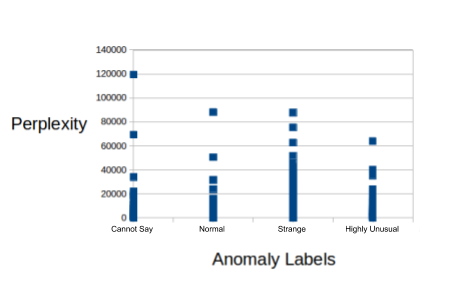
\includegraphics[width=4in]{figures/perplexity-comparison.png}
  \caption{Comparison of perplexity scores for different labels}
  \label{fig:nem_lm_ppl}
  \end{center}
\end{figure}

\section{Model for Semantic Anomaly Detection}
Neural Event Model (NEM) is a supervised model that learns to differentiate between anomalous and
normal events by 
classifying dense representations of events, otherwise known as event embeddings. We treat the problem as a binary classification problem, with
\textit{normal} and \textit{anomalous} being the two classes.
The event embeddings are computed using a structured composition model
that represents an event as the composition of the five slot-fillers: \textbf{action},
\textbf{agent}, \textbf{patient}, \textbf{time} and \textbf{location}.
Figure~\ref{fig:nem} shows the pipeline for anomalous event detection using NEM. We
first identify the fillers for the five slots mentioned above, by running a PropBank \citep{palmer2005proposition}
style Semantic Role Labeler (SRL). We use the following mapping of roles to obtain the event structure:
\begin{itemize}
 \item V $\rightarrow$ action
 \item A0 $\rightarrow$ agent
 \item A1 $\rightarrow$ patient
 \item AM-TMP $\rightarrow$ time
 \item AM-LOC $\rightarrow$ location
\end{itemize}
This structured input is then passed to NEM. The model has three components:

\paragraph{Argument Composition} This component encodes all the role fillers as vectors in the same space.
This is accomplished by embedding the words in each role filler, and then passing them through a Recurrent
Neural Network (RNN) with Long Short-Term Memory (LSTM) \citep{hochreiter1997long} cells. Note that the same LSTM is
used for all the slots. Concretely,
\begin{equation}
 a_s = \text{LSTM}(I_s)
\end{equation}
where $I_s$ denotes the ordered set of word vector representations in in the filler of slot $s$, and
$a_s$ represents the vector representation of that slot filler.

\paragraph{Event Composition} The slot filler representations are then composed using slot specific
projection weights to obtain a single event representation. Concretely,
\begin{align}
 \bar{a}_s &= \tanh(W_s^\intercal a_s + b_s) \quad \text{where } s \in \{c,g,p,t,l\} \\
 e &=  \bar{a}_c + \bar{a}_g + \bar{a}_p + \bar{a}_t + \bar{a}_l 
\end{align}
$W_s \in \mathbb{R}^{d \times d}$ and $b_s \in \mathbb{R}^{d}$ are slot specific projection weights and biases respectively, with $s$ denoting one of a\underline{c}tion,
a\underline{g}ent, \underline{p}atient, \underline{t}ime and \underline{l}ocation. $d$ is the dimensionality of the word embeddings.
Event composition involves performing non-linear projections of all slot-filler representations, and finally obtaining an event representation
$e$.

\paragraph{Anomaly Classification} The event representation is finally passed through a softmax layer to obtain
the predicted probabilities for the two classes.
\begin{align}
 p_e & = \text{softmax}(W_e^\intercal e + b_e) \\
\end{align}
$W_e \in \mathbb{R}^{d \times 2}$ and $b_e \in \mathbb{R}^2$ are the weight and bias values of the softmax layer respectively.
As it can be seen, the layer projects the event representation into a two-dimensional space before applying the softmax non-linearity.

\begin{figure}
  \begin{center}
  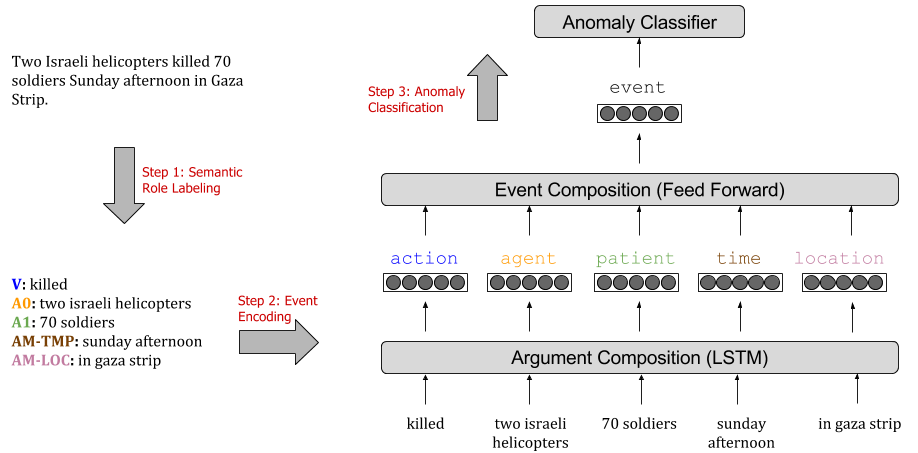
\includegraphics[width=6.5in]{figures/nem_pipeline.png}
  \caption{Anomaly Classification Pipeline with Neural Event Model}
  \label{fig:nem}
  \end{center}
\end{figure}

\subsection{Training}
Given the output from NEM, we define
\begin{align}
 p^1_e(\theta) &= P(\text{anomalous} | e; \theta) \\
 p^0_e(\theta) &= P(\text{normal} | e; \theta)
\end{align}
where $\theta$ are the parameters in the model and compute the label loss based on the prediction at the end of anomaly classification as a cross entropy loss as follows:
\begin{equation}
J(\theta) = - l \log p^1_e(\theta) + (1-l) \log p^0_e(\theta)
\end{equation}
where $l$ is the reference binary label indicating whether the event is normal or
anomalous. The three components of the model described above: argument composition, event composition and anomaly classification are all trained jointly.
That is, we optimize the following objective.
\begin{equation}
 \theta^* = \argmin_{\theta} J(\theta)
\end{equation}
where $\theta$ includes all $W_s$ and $b_s$ from all the slots, $W_e$ and $b_e$ from event composition and also all the LSTM parameters from argument composition.
We optimize this objective using ADAM \citep{kingma2014adam}. The model is implemented\footnote{The code is publicly available at \url{https://github.com/pdasigi/neural-event-model}}
using Keras \citep{chollet2015keras}. Note that the model described here is an extension of the one described in our previously published paper \citep{dasigi2014modeling}.
The main improvements here include using an LSTM-RNN as the encoder in argument composition instead of a simple RNN, and jointly training argument composition, event composition and anomaly classification,
whereas the older model included training argument composition separately using an unsupervised objective.

\section{Results}
We merged the two anomaly classes (strange and highly unusual) and calculated accuracy and F-score (for the anomaly class) of the binary
classifier. For the sake of comparison, we also define the following two baseline models.

\paragraph{PMI Baseline} We compare the performance of our model against a baseline that is based
on how well the semantic arguments in the event match the selectional preferences 
of the predicate.  We measure selectional preference using Point-wise Mutual Information
(PMI) \cite{church1990word} of the head words of each semantic argument with the predicate.  
The baseline model is built as follows.  We perform dependency parsing using MaltParser
\cite{nivre2007maltparser} on the sentences in the training data used in the first phase of training to
obtain the head words of the semantic arguments.  We then calculate the PMI values of all the pairs
$<h_A, p>$ where $h$ is the head word of argument $A$ and $p$ is the predicate of the event.  
For training our baseline classifier, we use the labeled training data from the event composition phase.
The features to this classifier are the PMI measures of the $<h_A, p>$ pairs estimated from the larger
dataset.  The classifier thus trained to distinguish between anomalous and normal events is applied to the test set.

\paragraph{LSTM Baseline} To investigate the importance of our proposed event representation, we also implemented a LSTM baseline that
directly encodes sentences. The following equations describe the model.
\begin{align}
 w &= \text{LSTM}(I) \\
 \bar{w} &= \tanh(W_w^\intercal w + b_w) \\
 p_u &= \text{softmax}(W_u^\intercal \bar{w} + b_u)
\end{align}
Note that this model is comparable in complexity, and has the same number of non-linear transformations as NEM. $\bar{w}$ represents a
word level composition instead of an argument-level composition in NEM, and $p_u$ is a probability distribution defined over an
\underline{u}nstructured composition as features. Training of this baseline model is done in the same way as NEM.

\begin{table}
\begin{center}
  \begin{tabular}[c]{|c|c|c|}
 \cline{2-3}
 \multicolumn{1}{c|}{}& \textbf{Accuracy} & \textbf{F-Score} \\
 \hline
 PMI Baseline& 45.2\% & 45.1\%\\
 LSTM Baseline & 82.5\% & 77.4\%\\
 \hline
 NEM & \textbf{84.9\%}& \textbf{79.7\%}\\
 \hline
  \end{tabular}
\end{center}
 \caption{Classification Performance and Comparison with Baselines}
 \label{table:nem_anomaly_results}
\end{table}

Table~\ref{table:nem_anomaly_results} shows the results and a comparison with the two baselines.  The accuracy of the 
baseline classifier is lower than 50\%, which is the expected accuracy of a classifier that assigns labels randomly.  
As seen in the table, the LSTM model proves to be a strong baseline, but it under performs in comparison with NEM,
showing the value of our proposed event composition model. The difference between the performance of
NEM and the LSTM baseline is statistically significant with $p < 0.0001$. Figure~\ref{fig:nem_roc} shows the ROC curves
for NEM and the LSTM baseline.
\begin{figure}
  \begin{center}
  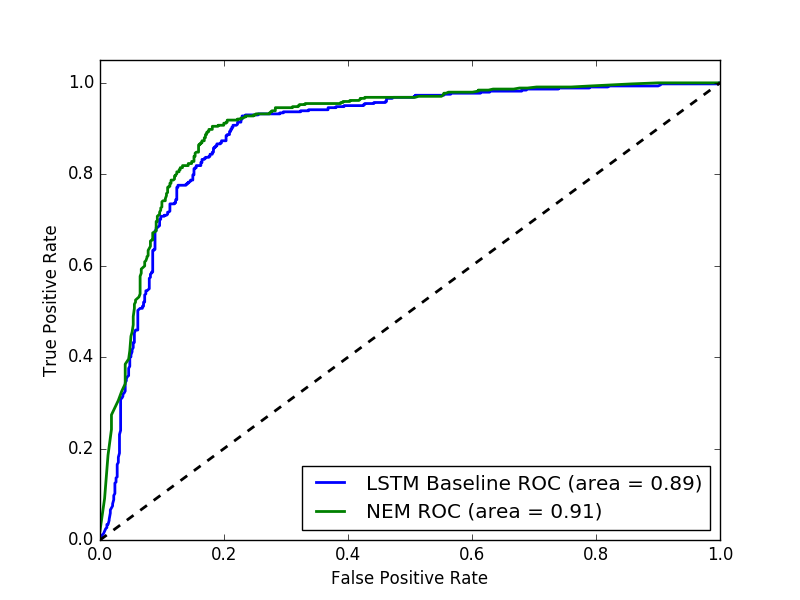
\includegraphics[width=4in]{figures/nem_roc.png}
  \caption{ROC curves for the LSTM baseline and NEM}
  \label{fig:nem_roc}
  \end{center}
\end{figure}


To further compare NEM with human annotators, we give to MACE, the binary predictions produced
by NEM, and those by the LSTM baseline along with the annotations and
measure the competence.  For the sake of comparison, we also give to MACE, a list of
random binary labels as one of the annotations 
to measure the competence of a hypothetical worker that made random choices. 
These results are reported in Table~\ref{table:nem_mace_competence}.
\begin{table}
\begin{center}
  \begin{tabular}[c]{|c|c|}
 \hline
 Human highest  & 0.896 \\
  Human average & 0.633 \\
  Human lowest & 0.144 \\
  \hline
  Random & 0.054 \\
  \hline
  LSTM Baseline & 0.743 \\
  NEM &  0.797 \\
  \hline
  \end{tabular}
\end{center}
 \caption{Anomaly Detection Competence}
 \label{table:nem_mace_competence}
\end{table}
Unsurprisingly, the competence of the random classifier is very low, and is worse than the least competent human.
It can be seen that MACE predicts both the LSTM baseline and NEM to be more competent than human average. This is an encouraging
result, especially given that this is a hard problem even for humans.

\section{Conclusion}
%TODO: Error analysis
In this chapter, we have looked at how selectional preferences can be leveraged to model events and represent
them in such a way as to distinguish anomalous events from normal events. Results from our controlled experiments
comparing the proposed model with one that directly encodes whole sentences have shown the value of using the proposed structured
composition.

The model we have shown in this chapter is just one instantiation of using selectional preferences to capture implicit knowledge.
In addition to some of the traditional uses of selectional preferences in dependency structures described in Section~\ref{sec:nem_background},
there also exists a large body of work in applications of selectional preferences to relations among entities. Knowledge base completion and 
relation extraction
\cite[among others]{mintz2009distant,sutskever2009modelling,nickel2011three,bordes2011learning,socher2013reasoning,gardner2014incorporating},
fall under this category.

There are limitations to the kind of implicit knowledge that selectional preferences over processed inputs can capture.
There is often an unmet need for encoding factual commonsense knowledge. 
For example, one important aspect of anomaly that is currently not handled by NEM
is the level of generality of the concepts the events contain.  Usually
more general concepts cause events to be more normal since they convey
lesser information.  For example, an American soldier shooting another American
soldier
may be considered unusual, while a soldier shooting another soldier may not be
as unusual, and at the 
highest level of generalization, a person shooting another person is normal. 
This information about generality can be incorporated into the event model only
by using real world knowledge from knowledge bases like Wordnet \cite{miller1995wordnet}. We pursue that direction
in Chapter~\ref{chapter:ontolstm}.
\chapter{Sentence Understanding with Background Knowledge from Ontologies}
\label{chapter:ontolstm}
In this chapter, we describe augmenting encoders with the kind of background
knowledge that is available in external knowledge sources.

The model shown here is one specific kind of knowledge augmented encoder. It is an
ontology-aware recurrent neural network, an encoder that computes token level 
word representations grounded in an ontology (Wordnet).
The kind of background knowledge we deal with here is that of various senses of
words, and the generalizations of the concepts that correspond to each sense.
We encode that information by using Wordnet to find the 
collection of semantic concepts manifested by a word type, and represent a word 
type as a collection of concept embeddings. We show
how to integrate the proposed ontology-aware lexical representation with 
recurrent neural networks (RNNs) to model token sequences.

\section{Ontology-Aware Token Embeddings}
\paragraph{Types vs. Tokens} In accordance with standard terminology, we make
the following distinction 
between types and tokens in this chapter: By word types, we mean the surface form 
of the word, whereas by tokens we mean the instantiation of the surface form in 
a context. For example, the same word type \textit{`pool'} occurs as two 
different tokens in the sentences \textit{``He sat by the pool,''} and 
\textit{``He played a game of pool.''}

Type-level word embeddings map a word type (i.e., a surface form) to a dense 
vector of real numbers such that similar word types have similar embeddings. 
When pre-trained on a large corpus of unlabeled text, they provide an effective 
mechanism for generalizing statistical models to words which do not appear in 
the labeled training data for a downstream task. Most word embedding models 
define a single vector for each word type. However, a 
fundamental flaw in this design is their inability to distinguish between 
different meanings and abstractions of the same word. In the two sentences shown 
above, the word \textit{`pool'} has different meanings, but the same 
representation is typically used for both of them. Similarly, the fact that 
\textit{`pool'} and \textit{`lake'} are both kinds of water bodies is not 
explicitly incorporated in most type-level embeddings.
Furthermore, it has become a standard practice to tune pre-trained word 
embeddings as model parameters during training for an NLP task 
\cite[e.g.,][]{chen:14,lample:16}, potentially allowing the parameters of a 
frequent word in the labeled training data to drift away from related but rare 
words in the embedding space. 

In this chapter, we represent a word token in a given context by estimating a 
context-sensitive probability distribution over relevant concepts in WordNet 
\citep{miller1995wordnet} and use the expected value (i.e., weighted sum) of the 
concept embeddings as the token representation.
Effectively, we map each word type to a grid of concept embeddings (see 
Fig.~\ref{fig:ontolstm_tensor}), which are shared across many words. The word 
representation is computed as a distribution over the concept embeddings from 
the word's grid. We show how these distributions can be 
learned conditioned on the context when the representations are plugged into 
RNNs.
Intuitively, commonsense knowledge encoded as WordNet relations could 
potentially help with language understanding tasks. 
but mapping tokens to entities in WordNet is a challenge. One needs to at least 
disambiguate the sense of the token before being able to use the relevant 
information. Similarly, not all the hypernyms defined by WordNet may be useful 
for the task at hand as some may be too general to be informative.
 
\begin{figure}[t]
\begin{center}
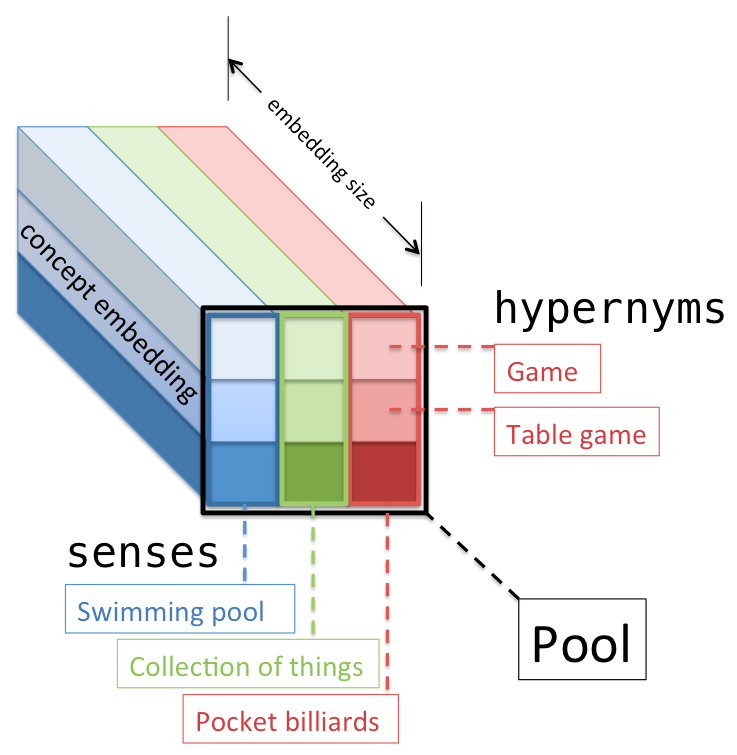
\includegraphics[width=3in]{figures/tensor2.png}
\caption{Example of ontology-aware lexical representation}
\label{fig:ontolstm_tensor}
\end{center}
\end{figure}

We take a task-centric approach towards doing this, and learn the token 
representations jointly with the task-specific parameters.
In addition to providing context-sensitive token embeddings, the proposed method 
implicitly regularizes the embeddings of related words by forcing related words 
to share similar concept embeddings. 
As a result, the representation of a rare word which does not appear in the 
training data for a downstream task benefits from all the updates to related 
words which share one or more concept embeddings. While the results presented in this thesis are from a model that relies on WordNet, 
and we exploit the order of senses given by WordNet, the approach is, in principle 
applicable to any ontology, with appropriate modifications. Here, we do not assume the inputs are 
sense tagged.

We evaluate the proposed embeddings in two applications. The first is predicting prepositional phrase 
(PP) attachments (see Section~\ref{sec:ontolstm_pp_model}), a challenging problem which 
emphasizes the selectional preferences between words in the PP and each of the 
candidate head words.  The second application is Textual Entailment (see Section~\ref{sec:ontolstm_snli}),
a task that benefits from hypernymy features from WordNet, providing generalization information.
Our empirical results and detailed analysis (see Section\ref{sec:ontolstm_pp_experiments} and Section~\ref{sec:ontolstm_pp_experiments}) show 
that the proposed embeddings effectively use WordNet to improve the accuracy of 
PP attachment predictions.

\section{Related Work}
\label{sec:ontolstm_related_work}
% concept embeddings
This work is related to various lines of research within the NLP community: dealing with synonymy and homonymy in word representations both in the context of distributed embeddings and more traditional vector spaces; hybrid models of distributional and knowledge based semantics; and selectional preferences and their relation with syntactic and semantic relations.

\subsection{Multi-prototype Word Vectors}
The need for going beyond a single vector per word-type has been well established for a while, and many efforts were focused on building multi-prototype vector space models of meaning \cite[][etc.]{reisinger2010multi,huang2012improving,chen2014unified,jauhar:15,neelakantan2015efficient,arora2016linear}. However, the target of all these approaches is obtaining multi-sense word vector spaces, either by incorporating sense tagged information or other kinds of external context. The number of vectors learned is still fixed, based on the preset number of senses. In contrast, our focus is on learning a context dependent distribution over those concept representations. Other work not necessarily related to multi-sense vectors, but still related to our work includes \cite{belanger:15}'s work which proposed a Gaussian linear dynamical system for estimating token-level word embeddings, and \cite{Vilnis2014WordRV}'s work which proposed mapping each word type to a density instead of a point in a space to account for uncertainty in meaning. These approaches do not make use of lexical ontologies and are not amenable for joint training with a downstream NLP task. 

Related to the idea of concept embeddings is \cite{rothe:15} who estimated WordNet synset representations, given pre-trained type-level word embeddings.
In contrast, our work focuses on estimating token-level word embeddings as context sensitive distributions of concept embeddings.

\subsection{Hybrid Models of Knowledge-based and Distributional Semantics}
There is a large body of work that tried to improve word embeddings using external resources. \cite{yu:14} extended the CBOW model \cite{mikolov:13} by adding an extra term in the training objective for generating words conditioned on similar words according to a lexicon.
\cite{jauhar:15} extended the skipgram model \cite{mikolov:13} by representing word senses as latent variables in the generation process, and used a structured prior based on the ontology.
\cite{faruqui:15} used belief propagation to update pre-trained word embeddings on a graph that encodes lexical relationships in the ontology.
Similarly, \cite{johansson2015embedding} improved word embeddings by representing each sense of the word in a way that reflects the topology of the semantic network they belong to, and then representing the words as convex combinations of their senses.
In contrast to previous work that was aimed at improving \textit{type level} word representations, we propose an approach for obtaining \textit{context-sensitive} embeddings at the \textit{token level}, while jointly optimizing the model parameters for the NLP task of interest.

\subsection{WordNet as a source for Selectional Preferences}
\cite{resnik:93} showed the applicability of semantic classes and selectional preferences to resolving syntactic ambiguity. \cite{Zapirain2013SelectionalPF} applied models of selectional preferences automatically learned from WordNet and distributional information, to the problem of semantic role labeling. \cite{resnik:93,brill1994rule,agirre2008improving} and others have used WordNet information towards improving prepositional phrase attachment predictions.

\section{WordNet-Grounded Context-Sensitive Token Embeddings}
\label{sec:ontolstm_input_rep}

In this section, we focus on defining our context-sensitive token embeddings. 
We first describe our grounding of word types using WordNet concepts.
Then, we describe our model of context-sensitive token-level embeddings as a weighted sum of WordNet concept embeddings. 

\subsection{WordNet Grounding}
We use WordNet to map each word type to a set of synsets, including possible generalizations or abstractions. 
Among the labeled relations defined in WordNet between different synsets, we focus on the hypernymy relation to help model generalization and selectional preferences between words, which is especially important for predicting PP attachments \citep{resnik:93}.
To ground a word type, we identify the set of (direct and indirect) hypernyms of the WordNet senses of that word.
A simplified grounding of the word `pool' is illustrated in Figure \ref{fig:ontolstm_wordnet_grounding}.
This grounding is key to our model of token embeddings, to be described in the following subsections. 

\subsection{Context-Sensitive Token Embeddings}
\label{sec:ontolstm_embedding_model}

Our goal is to define a context-sensitive model of token embeddings which can be used as a drop-in replacement for traditional type-level word embeddings.

\paragraph{Notation.}
Let $\textit{Senses}(w)$ be the list of synsets defined as possible word senses of a given \underline{w}ord type $w$ in WordNet, and $\textit{Hypernyms}(s)$ be the list of hypernyms for a \underline{s}ynset $s$.
\footnote{For notational convenience, we assume that $s \in \textit{Hypernyms}(s)$.} Figure~\ref{fig:ontolstm_wordnet_grounding} shows an example. In the figure, solid arrows
represent possible senses and dashed arrows represent hypernym relations. Note that the same set of concepts are used to ground the word \textit{`pool'} regardless of its context.
Other WordNet senses for \textit{`pool'} were removed from the figure for simplicity. According to figure, 
\begin{align}
\textit{Senses}&(\text{pool}) = [\text{pond.n.01, pool.n.09}], \text{and} \nonumber \\
\textit{Hypernyms}&(\text{pond.n.01}) = [\text{pond.n.01, lake.n.01}, \nonumber \\
&\text{body\_of\_water.n.01, entity.n.01}] \nonumber
\end{align}

\begin{figure}
\begin{center}
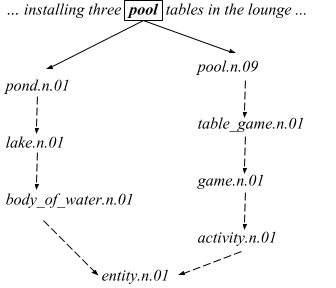
\includegraphics[width=3in]{figures/ontolstm_wordnet_grounding.png}
\caption{An example grounding for the word \textit{pool}}
\label{fig:ontolstm_wordnet_grounding}
\end{center}
\end{figure}
Each WordNet synset $s$ is associated with a set of parameters $\mathbf{v}_s \in \mathbb{R}^n$ which represent its embedding. 
This parameterization is similar to that of \cite{rothe:15}.

\paragraph{Embedding model.}

\begin{figure}[t]
\begin{center}
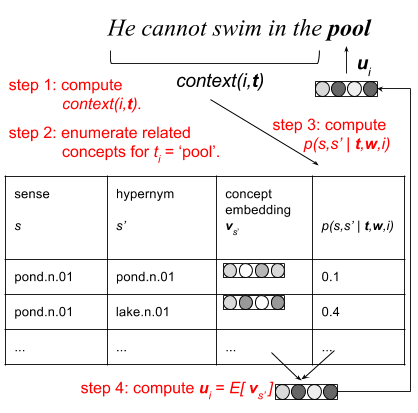
\includegraphics[width=3.5in]{figures/ontolstm_token_embedding.png}
\caption{Steps for computing the context-sensitive token embedding for the word \textit{`pool'}, as described in Section\ref{sec:ontolstm_embedding_model}.
\label{fig:ontolstm_token_embedding}}
\end{center}
\end{figure}

Given a sequence of \underline{t}okens $\boldsymbol{t}$ and their corresponding word types $\boldsymbol{w}$, let $\mathbf{u}_i  \in \mathbb{R}^n$
be the embedding of the word token $t_i$ at position $i$. Unlike most embedding models, the token embeddings $\mathbf{u}_i$ are not parameters.
Rather, $\mathbf{u}_i$ is computed as the expected value of concept embeddings used to ground the word type $w_i$ corresponding to the token $t_i$:
\begin{align}
\mathbf{u}_i = \sum_{s \in \textit{Senses}(w_i)} 
\sum_{s' \in \textit{Hypernyms}(s)}
p(s, s' \mid \boldsymbol{t}, \boldsymbol{w}, i) \  &\mathbf{v_{s'}} 
 \label{eq:ontolstm_token_embedding}\end{align}
such that
\begin{equation}
\sum_{s \in \textit{Senses}(w_i)} \sum_{s' \in \textit{Hypernyms}(s)} p(s, s' \mid \boldsymbol{t}, \boldsymbol{w}, i) = 1
\nonumber \end{equation}

The distribution which governs the expectation over synset embeddings factorizes into two components:
\begin{align}
p(s, s' \mid \boldsymbol{t}, \boldsymbol{w}, i) \propto& 
\lambda_{w_i} \exp^{-\lambda_{w_i} \  \textit{rank}(s, w_i)} \times \nonumber \\
&  \textit{MLP}( [\mathbf{v}_{s'}; \textit{context}(i, \boldsymbol{t})]) 
\label{eq:ontolstm_attention}
\end{align}
The first component, $\lambda_{w_i} \exp^{-\lambda_{w_i} \  \textit{rank}(s, w_i)}$, is a sense prior which reflects the prominence of each word sense for a given word type. Here, we exploit\footnote{Note that for ontologies where such information is not available, our method is still applicable but without this component.
We show the effect of using a uniform sense prior in Section~\ref{sec:ontolstm_pp_analysis}.} the fact that WordNet senses are ordered in descending order of their frequencies, obtained from sense tagged corpora, and parameterize the sense prior like an exponential distribution.
$rank(s, w_i)$ denotes the rank of sense $s$ for the word type $w_i$, thus $rank(s, w_i)=0$ corresponds to $s$ being the first sense of $w_i$.
The scalar parameter ($\lambda_{w_i}$) controls the decay of the probability mass, which is learned along with the other parameters in the model. Note that sense priors are defined for each word type ($w_i$), and are shared across all tokens which have the same word type.

$\textit{MLP}( [\mathbf{v}_{s'}; \textit{context}(i, \boldsymbol{t})])$, the second component, is what makes the token representations context-sensitive. 
It scores each concept in the WordNet grounding of $w_i$ by feeding the concatenation of the concept embedding and a dense vector that summarizes the textual context into a multilayer perceptron ($\textit{MLP}$) with two $tanh$ layers followed by a $softmax$ layer.
This component is inspired by the soft attention often used in neural machine translation \citep{bahdanau:14}.\footnote{Although soft attention mechanism is typically used to explicitly represent the importance of each item in a sequence, it can also be applied to non-sequential items.} The definition of the $\textit{context}$ function is dependent on the encoder used to encode the context.
We describe a specific instantiations of this function in Section~\ref{sec:ontolstm_pp_model} and Section~\ref{sec:ontolstm_snli}.

To summarize, Figure \ref{fig:ontolstm_token_embedding} illustrates how to compute the embedding of a word token $t_i=\textit{`pool'}$ in a given context:
\begin{enumerate}
    \item compute a summary of the context $\textit{context}(i, \boldsymbol{t})$,
    \item enumerate related concepts for $t_i$,
    \item compute $p(s,s'\mid \boldsymbol{t}, \boldsymbol{w}, i)$ for each pair $(s,s')$, and
    \item compute $\mathbf{u}_i = \mathbb{E}[\mathbf{v}_{s'}]$.
\end{enumerate}

In the following section, we describe our model for predicting PP attachments, including our definition for $\textit{context}$ for this problem.

\section{PP Attachment}
\label{sec:ontolstm_pp_model}
Disambiguating PP attachments is an important and challenging NLP problem. Since modeling hypernymy and selectional preferences is critical for successful prediction of PP attachments \citep{resnik:93}, it is a good fit for evaluating our WordNet-grounded context-sensitive embeddings.

\begin{figure}[t]
\begin{center}
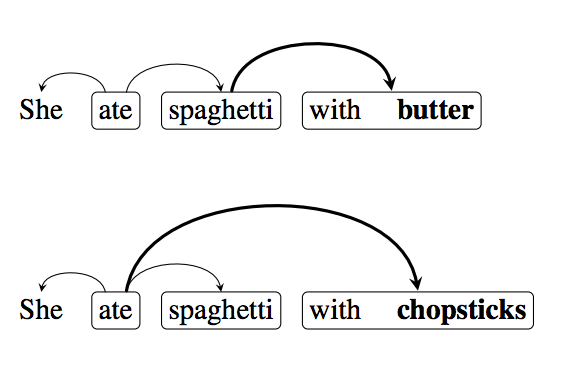
\includegraphics[width=3.2in]{figures/pp_attachment_example.png}
\label{fig:ontolstm_pp_example}
\caption{ Two sentences illustrating the importance
of lexicalization in PP attachment decisions.}
\end{center}
\end{figure}

Figure \ref{fig:ontolstm_pp_example}, reproduced from \cite{belinkov2014exploring}, illustrates an example of the PP attachment prediction problem.
In the top sentence, the PP \textit{`with butter'} attaches to the noun \textit{`spaghetti'}. 
In the bottom sentence, the PP \textit{`with chopsticks'} attaches to the verb \textit{`ate'}.
The accuracy of a competitive English dependency parser at predicting the head word of an ambiguous prepositional phrase is 88.5\%, significantly lower than the overall unlabeled attachment accuracy of the same parser (94.2\%).\footnote{See Table \ref{tab:ontolstm_parser_ppa_results} for detailed results.}

This section formally defines the problem of PP attachment disambiguation, describes our baseline model, then shows how to integrate the token-level embeddings in the model.

\subsection{Problem Definition}
\label{sec:ontolstm_pp_problem_definition}
We follow \cite{belinkov2014exploring}'s definition of the PP attachment problem.
Given a \underline{p}reposition $p$ and its direct \underline{d}ependent $d$ in the prepositional phrase (PP), our goal is to predict the correct head word for the PP among an ordered list of candidate \underline{h}ead words $\boldsymbol{h}$.
Each example in the train, validation, and test sets consists of an input tuple $\langle \boldsymbol{h}, p, d \rangle$ and an output index $k$ to identify the correct head among the candidates in $\boldsymbol{h}$. Note that the order of words that form each $\langle \boldsymbol{h}, p, d\rangle$ is the same as that in the corresponding original sentence.

\subsection{Model Definition}
Both our proposed and baseline models for PP attachment use bidirectional RNN with LSTM cells (bi-LSTM) to encode the sequence $\boldsymbol{t} = \langle h_1, \ldots, h_K, p, d \rangle$.

We score each candidate head by feeding the concatenation of the output bi-LSTM vectors for the head $h_k$, the preposition $p$ and the direct dependent $d$ through an MLP, with a fully connected $\textit{tanh}$ layer to obtain a non-linear projection of the concatenation, followed by a fully-connected $\textit{softmax}$ layer:

\begin{align}
p(h_k \text{is head}) = \textit{MLP}_{\textit{attach}}([&\textit{lstm\_out}(h_k);\nonumber \\
&\textit{lstm\_out}(p);\nonumber \\
&\textit{lstm\_out}(d)]) \label{eq:pp_model}
\end{align}
To train the model, we use cross-entropy loss at the output layer for each candidate head in the training set.
At test time, we predict the candidate head with the highest probability according to the model in Eq. \ref{eq:pp_model}, i.e.,
\begin{align}
\hat{k} = \arg\max_k p(h_k \text{is head} = 1).
\end{align}
This model is inspired by the Head-Prep-Child-Ternary model of \cite{belinkov2014exploring}. 
The main difference is that we replace the input features for each token with the output bi-RNN vectors.

We now describe the difference between the proposed and the baseline models. Generally, let $\textit{lstm\_in}(t_i)$ and $\textit{lstm\_out}(t_i)$ represent the input and output vectors of the bi-LSTM for each token $t_i \in \boldsymbol{t}$ in the sequence. The outputs at each timestep are obtained by concatenating those of the forward and backward LSTMs.

\paragraph{Baseline model.}
In the baseline model, we use type-level word embeddings to represent the input vector $\textit{lstm\_in}(t_i)$ for a token $t_i$ in the sequence. The word embedding parameters are initialized with pre-trained vectors, then tuned along with the parameters of the bi-LSTM and $\textit{MLP}_{\textit{attach}}$. We call this model \textbf{LSTM-PP}.

\paragraph{Proposed model.}
\label{sec:ontolstm_proposed_ppa_model}
In the proposed model, we use token level word embedding as described in Section\ref{sec:ontolstm_input_rep} as the input to the bi-LSTM, i.e., $\textit{lstm\_in}(t_i) = \mathbf{u}_i$. The context used for the attention component is simply the hidden state from the previous timestep. However, since we use a bi-LSTM, the model essentially has two RNNs, and accordingly we have two context vectors, and associated attentions. That is, $\textit{context}_f\textit{(i, \textbf{t})} = \textit{lstm\_in}(t_{i-1})$ for the forward RNN and $\textit{context}_b\textit{(i, \textbf{t})} = \textit{lstm\_in}(t_{i+1})$ for the backward RNN. Consequently, each token gets two representations, one from each RNN. The synset embedding parameters are initialized with pre-trained vectors and tuned along with the sense decay ($\lambda_{w}$) and MLP parameters from Eq. \ref{eq:ontolstm_attention}, the parameters of the bi-LSTM and those of $\textit{MLP}_{\textit{attach}}$. We call this model \textbf{OntoLSTM-PP}.

\subsection{Experiments}
\label{sec:ontolstm_pp_experiments} 

\paragraph{Dataset and evaluation.} We used the English PP attachment dataset created and made available by \cite{belinkov2014exploring}. The training and test splits contain 33,359 and 1951 labeled examples respectively. As explained in Section\ref{sec:ontolstm_pp_problem_definition}, the input for each example is 1) an ordered list of candidate head words, 2) the preposition, and 3) the direct dependent of the preposition.
The head words are either nouns or verbs and the dependent is always a noun. 
All examples in this dataset have at least two candidate head words.
As discussed in \cite{belinkov2014exploring}, this dataset is a more realistic PP attachment task than the RRR dataset \citep{ratnaparkhi1994maximum}.
The RRR dataset is a binary classification task with exactly two head word candidates in all examples.
The context for each example in the RRR dataset is also limited which defeats the purpose of our context-sensitive embeddings.

\paragraph{Model specifications and hyperparameters.} 
For efficient implementation, we use mini-batch updates with the same number of senses and hypernyms for all examples, padding zeros and truncating senses and hypernyms as needed.
For each word type, we use a maximum of $S$ senses and $H$ indirect hypernyms from WordNet.
In our initial experiments on a held-out development set (10\% of the training data), we found that values greater than $S=3$ and $H=5$ did not improve performance. We also used the development set to tune the number of layers in $\textit{MLP}_{\textit{attach}}$ separately for the \textit{OntoLSTM-PP} and \textit{LSTM-PP}, and the number of layers in the attention MLP in \textit{OntoLSTM-PP}.
When a synset has multiple hypernym paths, we use the shortest one. 
Finally, words types which do not appear in WordNet are assumed to have one unique sense per word type with no hypernyms. Since the POS tag for each word is included in the dataset, we exclude WordNet synsets which are incompatible with the POS tag.
The synset embedding parameters are initialized using the synset vectors obtained by running AutoExtend \citep{rothe:15} on 100-dimensional GloVe \citep{pennington2014glove} vectors for WordNet 3.1. We refer to this embedding as \textit{GloVe-extended}. Representation for the OOV word types in LSTM-PP and OOV synset types in \textit{OntoLSTM-PP} were randomly drawn from a uniform 100-d distribution. 
Initial sense prior parameters ($\lambda_w$) were also drawn from a uniform 1-d distribution.

\paragraph{Baselines.} In our experiments, we compare our proposed model, \textit{OntoLSTM-PP} with three baselines -- \textit{LSTM-PP} initialized with GloVe embedding, \textit{LSTM-PP} initialized with GloVe vectors retrofitted to WordNet using the approach of \cite{faruqui:15} (henceforth referred to as \textit{GloVe-retro}), and finally the best performing standalone PP attachment system from \cite{belinkov2014exploring}, referred to as \textit{HPCD (full)} in the paper. \textit{HPCD (full)} is a neural network model that learns to compose the vector representations of each of the candidate heads with those of the preposition and the dependent, and predict attachments. The input representations are enriched using syntactic context information, POS, WordNet and VerbNet \citep{kipper2008large} information and the distance of the head word from the PP is explicitly encoded in composition architecture. In contrast, we do not use syntactic context, VerbNet and distance information, and do not explicitly encode POS information.

\subsubsection{PP Attachment Results}
\begin{table}
    \centering
    \begin{tabular}{|l|c|c|c|c|}
    \hline
    \textbf{System} & \textbf{Initialization} & \textbf{Embedding} & \textbf{Resources} & \textbf{Test Acc.}\\
    \hline
    HPCD (full) & Syntactic-SG & Type & WordNet, VerbNet & 88.7 \\
    \hline
    LSTM-PP  & GloVe & Type & - & 84.3 \\
    LSTM-PP & GloVe-retro & Type & WordNet & 84.8 \\
    OntoLSTM-PP & GloVe-extended & Token & WordNet & \textbf{89.7} \\
    \hline
    \end{tabular}
    \caption{Prepositional Phrase Attachment Results with OntoLSTM}
    \label{tab:ontolstm_direct_ppa_results}
\end{table}
%We compare OntoLSTM-PP to two instantiations of LSTM-PP as well as the best performing .  In all systems, the word type embedding or synset embedding is tuned during training. 
Table \ref{tab:ontolstm_direct_ppa_results} shows that our proposed token level embedding scheme \textit{OntoLSTM-PP} outperforms the better variant of our baseline \textit{LSTM-PP} (with GloVe-retro intialization) by an absolute accuracy difference of 4.9\%, 
or a relative error reduction of 32\%.
\textit{OntoLSTM-PP} also outperforms \textit{HPCD (full)}, the previous best result on this dataset. \textit{HPCD (full)} is from the original paper, and it uses syntactic SkipGram. \textit{GloVe-retro} is GloVe vectors retrofitted \citep{faruqui:15} to WordNet 3.1, and \textit{GloVe-extended} refers to the synset embeddings obtained by running AutoExtend \citep{rothe:15} on GloVe.

Initializing the word embeddings with \textit{GloVe-retro} (which uses WordNet as described in \cite{faruqui:15}) instead of GloVe amounts to a small improvement, compared to the improvements obtained using \textit{OntoLSTM-PP}.
This result illustrates that our approach of dynamically choosing a context sensitive distribution over synsets is a more effective way of making use of WordNet.


\paragraph{Effect on dependency parsing.} Following \cite{belinkov2014exploring}, we used RBG parser \citep{lei2014low}, and modified it by adding a binary feature indicating the PP attachment predictions from our model. 

We compare four ways to compute the additional binary features: 1) the predictions of the best standalone system \textit{HPCD (full)} in \cite{belinkov2014exploring}, 2) the predictions of our baseline model \textit{LSTM-PP}, 3) the predictions of our improved model \textit{OntoLSTM-PP}, and 4) the gold labels \textit{Oracle PP}. 

Table \ref{tab:ontolstm_parser_ppa_results} shows the effect of using the PP attachment predictions as features within a dependency parser. 
We note there is a relatively small difference in unlabeled attachment accuracy for all dependencies (not only PP attachments), even when gold PP attachments are used as additional features to the parser.
However, when gold PP attachment are used, we note a large potential improvement of 10.46 points in PP attachment accuracies (between the PPA accuracy for \textit{RBG} and \textit{RBG + Oracle PP}), which confirms that adding PP predictions as features is an effective approach. 
Our proposed model \textit{RBG + OntoLSTM-PP} recovers 15\% of this potential improvement, while \textit{RBG + HPCD (full)} recovers 10\%, which illustrates that PP attachment remains a difficult problem with plenty of room for improvements even when using a dedicated model to predict PP attachments and using its predictions in a dependency parser.

We also note that, although we use the same predictions of the \textit{HPCD (full)} model in  \cite{belinkov2014exploring}\footnote{The authors kindly provided their predictions for 1942 test examples (out of 1951 examples in the full test set). In Table \ref{tab:ontolstm_parser_ppa_results}, we use the same subset of 1942 test examples.}, we report different results than  \cite{belinkov2014exploring}.
For example, the unlabeled attachment score (UAS) of the baselines \textit{RBG} and \textit{RBG + HPCD (full)} are 94.17 and 94.19, respectively, in Table \ref{tab:ontolstm_parser_ppa_results}, compared to 93.96 and 94.05, respectively, in \cite{belinkov2014exploring}.
This is due to the use of different versions of the RBG parser.\footnote{We use the latest commit (SHA: e07f74) on the GitHub repository of the RGB parser.}

\begin{table}
    \centering
    \begin{tabular}{|l|c|c|}
    \hline
    \textbf{System} & \textbf{Full UAS} & \textbf{PPA Acc.}\\
    \hline
    RBG               & 94.17 & 88.51 \\
    RBG + HPCD (full) & 94.19 & 89.59 \\
    RBG + LSTM-PP  & 94.14 & 86.35 \\
    RBG + OntoLSTM-PP & 94.30 & 90.11 \\
    RBG + Oracle PP & 94.60 & 98.97 \\
    \hline
    \end{tabular}
    \caption{Results from RBG dependency parser with features coming from various PP attachment predictors and oracle attachments. }
    \label{tab:ontolstm_parser_ppa_results}
\end{table}

\subsubsection{Analysis}
\label{sec:ontolstm_pp_analysis}
We now analyze different aspects of our model in order to develop a better understanding of its behavior.

\paragraph{Effect of context sensitivity and sense priors.} We now show some results that indicate the relative strengths of two components of our context-sensitive token embedding model. The second row in Table \ref{tab:ontolstm_pp_ablation_results} shows the test accuracy of a system trained without sense priors (that is, making $p(s|w_i)$ from Eq. \ref{eq:ontolstm_token_embedding} a uniform distribution), and the third row shows the effect of making the token representations context-insensitive by giving a similar attention score to all related concepts, essentially making them type level representations, but still grounded in WordNet. As it can be seen, removing context sensitivity has an adverse effect on the results.
This illustrates the importance of the sense priors and the attention mechanism.

It is interesting that, even without sense priors and attention, the results with WordNet grounding is still higher than that of the two LSTM-PP systems in Table ~\ref{tab:ontolstm_direct_ppa_results}.
This result illustrates the regularization behavior of sharing concept embeddings across multiple words, which is especially important for rare words.

\paragraph{Effect of training data size.}
Since \textit{OntoLSTM-PP} uses external information, the gap between the model and \textit{LSTM-PP} is expected to be more pronounced when the training data sizes are smaller. To test this hypothesis, we trained the two models with different amounts of training data and measured their accuracies on the test set. The plot is shown in Figure ~\ref{fig:ontolstm_pp_data_size_variation}. As expected, the gap tends to be larger at smaller data sizes. Surprisingly, even with 2000 sentences in the training data set, \textit{OntoLSTM-PP} outperforms \textit{LSTM-PP} trained with the full data set. 
When both the models are trained with the full dataset, \textit{LSTM-PP} reaches a training accuracy of 95.3\%, whereas \textit{OntoLSTM-PP} reaches 93.5\%. The fact that \textit{LSTM-PP} is overfitting the training data more, indicates the regularization capability of \textit{OntoLSTM-PP}.
\begin{figure}
\begin{center}
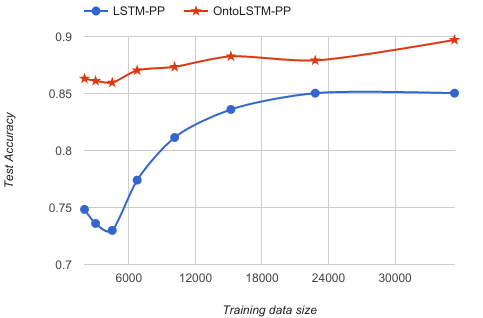
\includegraphics[width=3.6in]{figures/training_data_size.png}
\caption{Effect of training data size on test accuracies of OntoLSTM-PP and LSTM-PP.}
\label{fig:ontolstm_pp_data_size_variation}
\end{center}
\end{figure}

\begin{table}
    \centering
    \begin{tabular}{|l|c|}
    \hline
    \textbf{Model}	& \textbf{PPA Acc.}\\
    \hline
    full		& 89.7 \\
    - sense priors	& 88.4 \\
    - attention		& 87.5 \\
    \hline
    \end{tabular}
    \caption{Effect of removing sense priors and context sensitivity (attention) from the model.}
    \label{tab:ontolstm_pp_ablation_results}
\end{table}

\begin{figure*}
\begin{center}
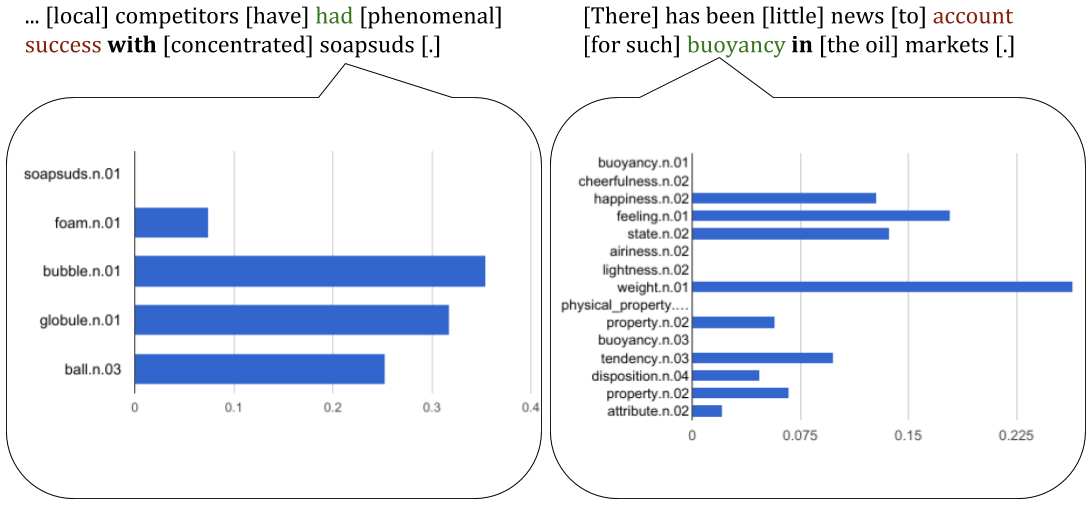
\includegraphics[width=6.2in]{figures/ontolstm_relative_attention.png}
\caption{Visualization of soft attention weights assigned by OntoLSTM to various synsets in Preposition Phrase Attachment}
\label{fig:ontolstm_pp_attention_visualization}
\end{center}
\end{figure*}
\paragraph{Qualitative analysis.} To better understand the effect of WordNet grounding, we took a sample of 100 sentences from the test set whose PP attachments were correctly predicted by OntoLSTM-PP but not by LSTM-PP. 
A common pattern observed was that those sentences contained words not seen frequently in the training data. Figure ~\ref{fig:ontolstm_pp_attention_visualization} shows two such cases where OntoLSTM-PP predicts the head correctly and
LSTM-PP does not, along with weights by OntoLSTM-PP to synsets that contribute to token representations of infrequent word types.
The prepositions are shown in bold, LSTM-PP's predictions in red and OntoLSTM-PP's predictions in green. Words that are not candidate heads or dependents are shown in brackets.
In both cases, the weights assigned by OntoLSTM-PP to infrequent words are also shown. The word types \textit{soapsuds} and \textit{buoyancy} 
do not occur in the training data, but OntoLSTM-PP was able to leverage the parameters learned for the synsets that contributed to their token representations.
Another important observation is that the word type \textit{buoyancy} has four senses in WordNet (we consider the first three), none of which is the metaphorical sense that is applicable to \textit{markets} as shown in the example here. Selecting a combination of relevant hypernyms from various senses may have helped OntoLSTM-PP make the right prediction. This shows the value of using hypernymy information from WordNet. Moreover, this indicates the strength of the hybrid nature of the model, that lets it augment ontological information with distributional information.

\paragraph{Parameter space.} We note that the vocabulary sizes in OntoLSTM-PP and LSTM-PP are comparable as the synset types are shared across word types. 
In our experiments with the full PP attachment dataset, we learned embeddings for 18k synset types with OntoLSTM-PP and 11k word types with LSTM-PP. Since the biggest contribution to the parameter space comes from the embedding layer,
the complexities of both the models are comparable.

\section{Textual Entailment}
\label{sec:ontolstm_snli}
We evaluate the capability of OntoLSTM to learn useful generalizations of concepts by testing it on
the task of textual entailment. We use the Stanford Natural Language Inference (SNLI) dataset \citep{bowman:15}.

\subsection{Data preprocessing} Since the dataset does not contain POS tag information unlike the PP attachment dataset,
we run Stanford's POS tagger \citep{toutanova:03} on the dataset.
To construct the tensor representation, we map the POS-tagged word to the first 
two synsets in WordNet (i.e. $S=2$), and extract the most direct five hypernyms 
(i.e., $H=5$). When a synset has multiple hypernym paths, we use the shortest 
one. In preliminary experiments, we found that using more word senses or more 
hypernyms per word sense does not improve the performance.
Like with the PPA dataset, words which do not appear in WordNet are assumed to
have one unique synset per word type with no hypernyms.

\subsection{Problem Definition}
Given a pair of sentences (premise and hypothesis), the model predicts one of 
three possible relationships between the two sentences: \textit{entailment}, 
\textit{contradiction} or \textit{neutral}.
We use the standard train, development and test splits of the SNLI corpus, which 
consists of 549K, 10K and 10K labeled sentence pairs, respectively.
For example, the following sentence pair is labeled \textit{entailment}:
 \begin{itemize}
  \item \textbf{Premise} \textit{Children and parents are splashing water at the 
pool.}
  \item \textbf{Hypothesis} \textit{Families are playing outside.}
 \end{itemize}
 
\subsection{Model Definition}
Following \cite{bowman2016fast}, our model for textual entailment uses two LSTMs with tied parameters
to  read the premise and the hypothesis of each example, then compute the vector $h$ 
which summarizes the sentence pair as the following concatenation (originally proposed by \cite{mou2015recognizing}):
$$h=\big[h_{\text{pre}}; h_{\text{hyp}}; h_{\text{pre}} 
-h_{\text{hyp}};h_{\text{pre}} *h_{\text{hyp}}\big]$$
where $h_\text{pre}$ is the output hidden layer at the end of the premise token 
sequence, $h_\text{hyp}$ is the output hidden layer at the end of the hypothesis 
token sequence.
The summary $h$ then feeds into two fully connected ReLU layers of size 1024, 
followed by a softmax layer of size 3 to predict the label.
The word embeddings and concept embeddings are of size 300, and the hidden 
layers 150.

The proposed model uses the WordNet grounded token embeddings, and we call it \textbf{OntoLSTM-TE}.
We compare it with two baselines: The first one is a simpler variant of \textit{OntoLSTM-TE}, and does not
use attention over synsets. We call it $\textbf{OntoLSTM-TE}_{\textbf{uni}}$. The second uses type level word representations, and 
we call it \textbf{LSTM-TE}.

The models are trained to maximize log-likelihood of correct labels in the 
training data, using ADAM \citep{kingma2014adam} with early stopping (up to 
twenty epochs).

\subsection{Experiments}
Table~\ref{tab:ontolstm_snli_results} shows the classification results. We also 
report previously published results of a similar neural architecture as an extra 
baseline: the 300-dimensional LSTM RNN encoder model in 
\cite{bowman2016fast}.\footnote{We note this is not the state of the art
on this dataset. This is the simplest sentence encoding based model for this task.}
They use GloVe as pretrained word embeddings while we jointly learn word/concept 
embeddings in the same model.
\cite{bowman2016fast}'s LSTM outperforms \textit{LSTM-TE} model by 0.9 absolute points 
on the test set. This may be due to the difference in input representations. 
Since we learn the synset representations in \textit{OntoLSTM-TE}, comparison with our LSTM 
implementations is more sensible.
The \textit{OntoLSTM-TE} outperforms \textit{LSTM-TE} by 1.4 absolute 
points on the test set, illustrating the utility of the ontology-aware word 
representations in a controlled experiment.

\begin{table}
    \centering
    \begin{tabular}{|l|c|c|c|}
    \hline
    \textbf{Model} & \textbf{GloVe} & \textbf{Train} & \textbf{Test}\\
    \hline
    LSTM-TE                        & No & 90.5 & 79.7 \\
    $\text{OntoLSTM-TE}_\text{uni}$  & No & 90.6 & 81.0 \\
    OntoLSTM-TE  & No & 90.5 & 81.1 \\ \hline
    LSTM (Bowman et al.) & Yes & 83.9 & 80.6 \\
    \hline
    \end{tabular}
    \caption{Results of OntoLSTM on the SNLI dataset}
    \label{tab:ontolstm_snli_results}
\end{table}


\subsection{Analysis}
\label{sec:ontolstm_snli_discussion}
\begin{figure}
\begin{center}
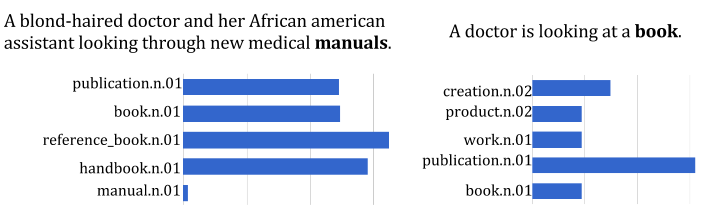
\includegraphics[width=5in]{figures/ontolstm_snli_comparison.png}
\caption{Visualization of soft attention weights assigned by OntoLSTM to various synsets in Textual Entailment}
\label{fig:ontolstm_snli_visualization}
\end{center}
\end{figure}

\paragraph{Generalization attention:} \label{sec:ontolstm_snli_generalization}
Fig.~\ref{fig:ontolstm_snli_visualization} shows one example from the test set of the 
SNLI dataset where hypernymy information is useful. 
The \textit{LSTM-TE} model shares no parameters between the lexical representations of 
\textit{book} and \textit{manuals}, and fails to predict the correct 
relationship (i.e., entailment). 
However, \textit{OntoLSTM-TE} leverages the fact that \textit{book} 
and \textit{manuals} share the common hypernyms \textit{book.n.01} and 
\textit{publication.n.01}, and assigns relatively high attention probabilities 
to these hypernyms, resulting in a similar lexical representation of the two 
words, and a correct prediction of this example.

The following is an example that \textit{LSTM-TE} gets right and \textit{OntoLSTM-TE} does not:
\begin{itemize}
 \item Premise: \textit{Women of India performing with blue streamers, in 
beautiful blue costumes.}
 \item Hypothesis: \textit{Indian women perform together in gorgeous costumes}
\end{itemize}
\textit{Indian} in the second sentence is an adjective, and \textit{India} in 
the first is an noun. By design, WordNet does not link words of different parts 
of speech. Moreover, the adjective hierarchies in WordNet are very shallow and 
\textit{gorgeous} and \textit{beautiful} belong to two different synsets, both 
without any hypernyms. Hence \textit{OntoLSTM-TE} could not use any generalization 
information in this problem.

\paragraph{Parameter space:} As mentioned earlier in the case of PP attachment problem,
the model size in \textit{LSTM-TE} and both variants of \textit{OntoLSTM-TE} are comparable
(11.1M and 12.7M parameters, respectively).

\section{Conclusion}
In this chapter, we showed a grounding of lexical items which acknowledges the semantic ambiguity 
of word types using WordNet and a method to learn a context-sensitive distribution over their representations.
We also showed how to integrate the proposed representation with recurrent neural networks for modeling sentences,
showing that the proposed WordNet-grounded context-sensitive token embeddings outperforms standard type-level embeddings
for predicting PP attachments and textual entailment.

We encoded a specific kind of background knowledge using WordNet in this work, but the methods described here can be extended 
to other kinds of structured knowledge sources as well. For example, one can effectively encode entities in text, using structured information
from Freebase. Such a model may help tasks like factual question answering.

One potential issue with the approach suggested in this chapter is
linking ambiguity. That is, deciding which entities in the background knowledge base, or concepts in the background ontology can be linked to
the tokens in the input utterance. In this chapter, we did not have to deal with this issue because linking words to WordNet concepts is a
trivial process. However, when extending this method to other kinds of knowledge bases, one may need to perform explicit entity or concept linking.
\part{Reasoning over Explicit Knowledge}
\chapter{Semantic Parsing over Semi-Structured Tables}
\label{chapter:neural_semantic_parsing}
So far we have evaluated our NLU pipelines by measuring the accuracy of the prediction component at any given task. The encoder component has not been explicitly evaluated.
This is because we generally view NLU pipelines as end-to-end systems, and do not care about the quality of the encoding as long as it serves as good features for the prediction
component. In this chapter, we take a different view and try to evaluate the encoder by investigating how well the encoded representations can be transferred across tasks. Transfer
learning in NLU systems is an attractive line of investigation for various reasons:
\begin{itemize}
 \item Not all language understanding tasks come with lots of training data. For some tasks it may be very difficult to get high quality annotations from humans due to factors such as 
 the task being subjective or requiring domain expertise. Being able to pre-train encoders on one task that has large amounts of training data available (like SNLI \cite{bowman:15} for textual entailment), and use them for similar
 tasks like paraphrasing or question answering, can address this issue.
 \item From a language understanding perspective, the transferability of the encoders gives us a clearer idea of what kind of features they are learning.
 \item Due to the large number of parameters involved, deep neural networks are highly prone to overfitting to the task. Transfer learning can address this problem. 
\end{itemize}

Transfer learning in neural networks has been well-studied for vision related problems. It has been shown \citep{zeiler2014visualizing} that object recognition models trained on
ImageNet \citep{deng2009imagenet} can be transfered to other object recognition datasets when the final classifier is retrained to the new dataset. A systematic study of the generality
of features learned at various layers in deep neural networks trained on natural images was done by \cite{yosinski2014transferable}. For language related problems, there do not exist similar studies.
There are however multi-task learning efforts for NLP tasks.  A notable example is the work by \cite{collobert2011natural} that showed the benefit of multi-task learning for surface-level NLP tasks 
like Named Entity Recognition, Part of Speech Tagging and Semantic Role Labeling. In this chapter, we investigate the transferability of the encoder in an NLU system trained on one task, to other similar tasks.

\section{Proposed Work}
The proposed work in this area involves answering the following concrete questions.
\begin{enumerate}
 \item Can different NLU tasks be jointly learned using the same neural network architecture?
 \item In a scenario where the NLU system is pretrained on a task with large amounts of data, how does the complexity (in terms of number of parameters)
 of the encoder affect its transferability to other tasks?
 \item How do external knowledge inputs affect the transferability of the encoder?
\end{enumerate}

\chapter{Proposed Work: Context Retrieval for Memory Networks}
\label{chapter:memnet_qa}
We consider the problem of reasoning over unstructured contexts in this chapter, and propose to build a model that can jointly retrieve and
reason over them.

\section{Memory Networks}
%TODO: General introduction about the need for explicit memory.
Memory Networks (MemNet) are a class of models
that combine inference with long-term memory. Unlike Recurrent Neural Networks
(RNN) that model language \citep{mikolov2010recurrent}, and their variants with
Long Short-Term Memory (LSTM) \citep{hochreiter1997long}, MemNets have an explicit
memory component with read and write functions. While the original MemNet model 
proposed by \cite{weston2014memory}, MemNN required explicit supervision
for selecting the relevant parts of the memory, \citep{sukhbaatar2015end}
proposed a end-to-end variant (MemN2N) where the memory selection component is
trained jointly with the rest of the network. These were previously used for
answering questions that require reasoning over multiple context sentences,
both in simulated \citep{bordes2010towards} and large-scale
\citep{fader2013paraphrase} scenarios.

In this chapter, we use the term \textit{memory network},
or the abbreviation \textit{MemNet}, to refer to any neural network model with an explicit memory component
that can be read from or written to. Our focus is mostly on the general class of models. Wherever necessary,
we refer to the original memory network model
proposed by \cite{weston2014memory} as \textit{MemNN} and the end to end model by \cite{sukhbaatar2015end}
as MemN2N.


\begin{figure*}
\begin{center}
  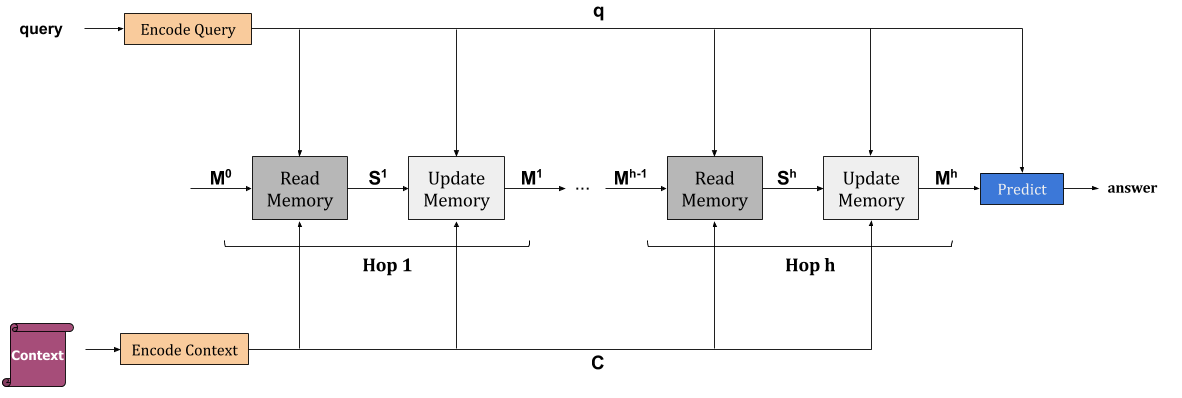
\includegraphics[width=7in]{figures/memory_network_generic.png}
  \caption{Schematic showing a generic view of memory networks}
  \label{fig:memnet}
  \end{center}
\end{figure*}
Figure~\ref{fig:memnet} shows the setup of a generic MemNet. It
takes as inputs:
\begin{itemize}
 \item a set of $N$ context sentences, indexed as $\{context_i\}_{i=1}^N$,
such that $context_i$ is a vector containing the indices of words in the $i^\text{th}$ sentence.
  \item a query, a single sentence indexed similar to context.
\end{itemize}

The sentences are then encoded using the \texttt{EncodeContext} and \texttt{EncodeQuery}
functions to produce the matrix $\textbf{C}$ and $\textbf{q}$ respectively.

The memory network then reasons over the context, represented \textbf{C}, given the 
query, represented by \textbf{q} over multiple memory layers, corresponding to multiple hops $i \in \{1, \ldots, h\}$.
At each hop, a memory layer performs two actions:
\begin{itemize}
 \item \texttt{ReadMemory} gets as input either the context ($\textbf{C}$) (in the first hop) or an updated memory representation ($\textbf{M}^i$)
 (in subsequent hops), and the query representation ($\textbf{q}$) to produce a summary of the memory $\textbf{S}^{i+1}$.
 \item \texttt{UpdateMemory} produces an updated memory representation ($\textbf{M}^{i+1}$) given the summary ($\textbf{S}^i$) and the query ($\textbf{q}$).
\end{itemize}

Finally, an answer is
predicted by passing the query encoding $\textbf{q}$, and the memory state at the
last hop ($\textbf{M}^h$) to the \texttt{Predict} function.

It can be seen that MemN2N fits into this setup with the following
configuration:
\begin{flalign}
&\texttt{EncodeQuery}(\text{query}) = \text{BOWEncoder}_q(\text{query}) \in \mathbb{R}^{d}\\
&\texttt{EncodeContext}(\text{Context}) = \text{BOWEncoder}_c(\text{Context}) \in \mathbb{R}^{N \times d}\\
&\texttt{ReadMemory}(\textbf{q}, \textbf{M}^{i-1}, \textbf{C}) = \text{softmax}(\textbf{C}.\textbf{M}^{i-1}).\textbf{C} \in \mathbb{R}^d\\
&\texttt{UpdateMemory}(\textbf{q}, \textbf{S}^i, \textbf{C}) = \textbf{q} + \textbf{S}^i \in \mathbb{R}^d \\
&\texttt{Predict}(\textbf{q}, \textbf{M}^h) = \text{softmax}(W.\textbf{M}^h) \in \mathbb{R}^o
\end{flalign}

where $\text{BOWEncoder}_q(.)$ and $\text{BOWEncoder}_c(.)$ are simply bag of
words models that aggregate the vector representations of all the words given by
the indices in the input and average them. $W \in \mathbb{R}^{o \times d}$ is a parameter of the
answer prediction function, causing the softmax to be over the output vocabulary size
$o$. Note that in MemN2N, \textbf{q} is not used in \texttt{ReadMemory} and \texttt{Predict}, and
\textbf{C} is not used in \texttt{UpdateMemory} since MemN2N is one of the simplest forms of MemNets.

In contrast, Gated Attention Reader \cite{dhingra2016gated} is relatively more complex, and uses the following
configuration:

\begin{flalign}
&\texttt{EncodeQuery}(\text{query}) = \text{Bi-GRU}_q(\text{query}) \in \mathbb{R}^d\\
&\texttt{EncodeContext}(\text{Context}) = \text{Bi-GRU}_c(\text{Context}) \in \mathbb{R}^{N_w \times d}\\
&\texttt{ReadMemory}(\textbf{q}, \textbf{M}^{i-1}, \textbf{C}) = \text{softmax}(\textbf{M}^{i-1}.\textbf{q}).\textbf{M}^{i-1} \in \mathbb{R}^{N_w \times d}\\
&\texttt{UpdateMemory}(\textbf{q}, \textbf{S}^i, \textbf{C}) = \text{Bi-GRU}_c(\textbf{S}^i.\textbf{q}) \in \mathbb{R}^{N_w \times d} \\
&\texttt{Predict}(\textbf{q}, \textbf{M}^h) = \text{softmax}(\textbf{M}^h.q) \in \mathbb{R}^{N_w}
\end{flalign}

The encoders used here are bidirectional Recurrent Neural Networks with Gated Recurrent Units \cite{cho2014learning}. Note that the output of $\text{Bi-GRU}_c$
is a matrix because it returns outputs from all time steps as a sequence. $N_w$ here denotes the number of tokens in all $N$ sentences in context. The output
produced here is a probability distribution over all tokens in the context, because this model was proposed for tasks that involve directly selecting a token from
the context.

Both the models described here assume that the context is well defined and small enough to fit in memory.
In this chapter, we focus on problems where these assumptions do not hold true, and where the context
be retrieved from a big corpus. Accordingly, we propose to add an additional
\texttt{RetrieveContext} module to our generic MemNet architecture.
Particularly, we are interested in developing MemNet models that
can figure out whether the available context is sufficient to make a prediction. We first
describe a target dataset for our model, and then list the issues we propose to address.

\section{Retrieval for Question Answering}
The datasets we use here are significantly different from the
QA datasets previously used to test memory networks, and require more complex
reasoning. One example of such question is shown below.
%TODO(pradeep): Make this a table?
\begin{itemize}
\item Astronauts weigh more on Earth than they do on the moon because
\begin{enumerate}[(a)]
 \item they have less mass on the moon
 \item their density decreases on the moon
 \item the moon has less gravity than Earth
 \item the moon has less friction than Earth
\end{enumerate}
\end{itemize}
%TODO(pradeep): Say more things about the nature of the problem.
The text relevant to questions like this may contain a single sentence that
has the information to answer this question, like this:
\begin{itemize}
 \item People weigh more on some planets than others because of differences in gravity.
\end{itemize}

Or it may span multiple sentences like this:
\begin{itemize}
 \item Moon's gravity is less than that of Earth.
 \item Weight of a person depends on the gravity of the planet.
\end{itemize}

Or in other cases, the text may not contain the relevant answer at all. Hence, this setup
requires a module in addition to the ones mentioned, that retrieves relevant content from
the corpus. However, as the size of the context increases, it becomes more and more expensive to reason over
it. Also, increased context size may add noise to prediction process. Hence, it is important to
retrieve context conservatively, and the model should reason whether the retrieved context
is sufficient to produce an answer.

\paragraph{Question Answering as Textual Entailment} In our proposed setup, we
cast the problem of deciding whether the given context is sufficient to answer the question, as a
textual entailment problem. That is, given a multiple choice question with answer options, we
convert the combination of the question and each of the options into a
statement, and check whether the statement can be entailed from relevant
background information. Given this setup, the \texttt{Predict} function
essentially becomes an entailment function. If none of the question-option combinations
can be entailed from (or contradicted by) the retrieved context, we retrieve more context.

\subsection{Proposed Algorithm}
Based on the ideas described so far, we now present the proposed algorithm, \textsc{AdaptiveRead}
to read and reason, while choosing to retrieve or predict depending on the sufficiency
of the context available.

\begin{algorithm}[H]
 \KwIn{$L$: large corpus, $q$: question}
 \KwOut{$a$: answer}
 $ContextSize = k$ \;
 $C = \texttt{RetrieveContext}(q, L, ContextSize)$, the top $k$ relevant sentences from the corpus\;
 \While{$ContextSize < MaxContextSize$} {
  \eIf{$\texttt{EntailsOrContradicts}(C, q)$}{
    $a = \texttt{Predict}(C, q)$ \;
    return $a$
  }{
    $ContextSize += k$ \;
    $C = \texttt{RetrieveContext}(q, L, ContextSize)$ \;
  }
 }
 \caption{\textsc{AdaptiveRead} algorithm that learns when to stop retrieving context}
\end{algorithm}

This algorithm shares some similarities with the \textit{ReasoNet} model
proposed by \cite{shen2016reasonet}, but the main difference is that while ReasoNet learns to
stop performing additional hops, the proposed algorithm learns to stop retrieving additional context.

\subsection{Potential Issues}
We identify the following potential issues in building \textsc{AdaptiveRead}.
\begin{enumerate}
 \item \textbf{Scalability to large corpora}: Depending on the complexity of \texttt{ReadMemory}, reasoning
 over large corpora may prove to be intractable. Earlier work in solving this problem involves building
 hierarchical models \citep{chandar2016hierarchical,choi2016hierarchical}. While \cite{chandar2016hierarchical}
 build a hierarchical memory network that uses a simple dot product for \texttt{RetrieveContext} and \texttt{ReadMemory},
 and thus use maximum inner product search (MIPS) to do them efficiently, \cite{choi2016hierarchical} perform summarization
 to retrieve context followed by answer prediction. We can use some of their ideas to make \texttt{RetrieveContext} a simpler
 process, and \texttt{ReadMemory} a more expensive one.
 
 \item \textbf{Difficulty in training}: Clearly, \textsc{AdaptiveRead} makes a hard choice between retrieving context and
 predicting an answer, thus making it impossible to train the model end-to-end using back-propagation. \cite{shen2016reasonet}
 and \cite{choi2016hierarchical} get around similar problems that involve hard choices by training with 
 REINFORCE \citep{williams1992simple} algorithm. However, REINFORCE is known to be unstable due to high variance induced by
 sampling.
\end{enumerate}


% \subsection{Preliminary Results}
% We performed some preliminary experiments to understand the 
% We now show some preliminary results of our memory network implementation on science question answering using MemN2N architecture with following change in configuration:
% \begin{flalign*}
% &\texttt{PredictAnswer}(u_0, s^H) = \texttt{HeuristicMatch}(u_0, s_h)
% \end{flalign*}
% where \texttt{HeuristicMatch}(.) is the heuristic matching function proposed by \cite{mou2015recognizing} for textual entailment, also used for our experiments with SNLI data in 
% Chapter~\ref{chapter:ontolstm}. The dataset used for these experiments is questions collected from 4th and 8th grade science text books.
% Context for each question was obtained as follows. We built a Lucene index over a big collection of sentences related to general science from various sources and extracted relevant background sentences for each question by querying it. For each of the
% options, we query the Lucene index with a combination of the option text and the question. We thus transform questions like the one shown above into four entailment problems where the combination of the
% question and one of the options is the hypothesis and the relevant background sentences are the premises. The final answer is picked by selecting the option (combined with the question) that has the highest
% entailment score. This is done by passing the final entailment scores through a softmax layer.
% 
% Preliminary results using our model are shown in Table~\ref{tab:memnet_qa_results}, using two different encoders
% to encode the input sentences and background. We also show the accuracy of a baseline system based on Lucene, that selects for every question, the option that results in the highest relevance score in the process
% described above for retrieving background sentences. It can be seen that the simple baseline does better than the memory network model.
% 
% \begin{table}
%     \centering
%     \begin{tabular}{|l|c|}
%     \hline
%     \textbf{Encoder} & \textbf{Test Acc.}\\
%     \hline
%     BOW & \% \\
%     GRU & 38.8\% \\
%     \hline
%     \hline
%     \textbf{Lucene baseline} & 41.1\% \\
%     \hline
%     \end{tabular}
%     \caption{Results of our Memory Network on ScienceQA in comparison with a Lucene baseline}
%     \label{tab:memnet_qa_results}
% \end{table}
% 
% \subsection{Analysis}
% 
% \subsection{Proposed Work}



\chapter{Summary and Timeline}


\section{Summary}
In this thesis we identified two classes of knowledge relevant to language
understanding: \textit{background} and \textit{contextual}.

We defined background knowledge as the implicit shared human knowledge that is
often omitted in human generated text or speech. We presented two ways to
incorporate this kind of knowledge in NLU systems.  In Chapter~\ref{chapter:ontolstm},
we explored how knowledge stated in an explicit symbolic knowledge base can be
incorporated in an NLU system to produce better encoded representations.
Particularly, we linked words to an ontology (WordNet),
and built an ontology-aware encoder that exploited the WordNet
hierarchies to learn context-sensitive token representations of words. We showed
the proposed model helps textual entailment and prepositional phrase attachment
tasks. By giving the encoder access to the hypernym paths of relevant concepts
we showed that we can learn useful task-dependent generalizations using an
attention mechanism.
Then in Chapter~\ref{chapter:nem}, we noted that not all background knowledge
can be stated symbolically, and focused on the kind of background knowledge that
is implicit in relations between linguistic elements. Concretely, we showed how selectional
preferences in structures relevant to the task at hand can be leveraged to
encode background knowledge. We showed that this is indeed more effective than
encoding whole sentences using comparable neural network architectures. 

We defined contextual knowledge as the explicit additional information that
reading comprehension systems need to ground reasoning in the respective
contexts. We focused on a subclass of reasoning tasks where reasoning can be
broken down into a sequence of discrete operations over structured contexts. We
viewed such problems as semantic parsing into domain-specific languages.
Given this framework, we pursued four research goals related to incorporating
contextual knowledge into semantic parsers, the first two related to the model
architecture while building transition based semantic parsers using neural encoder-decoder
models, and the remaining two related to the learning algorithms used when only weak
supervision is available. First, in Chapter~\ref{chapter:wikitables}, we investigated how the
knowledge of syntactic and semantic properties of the domain specific language
can be exploited to restrict the search space of the decoder in an
encoder-decoder model built for semantic parsing. Second, also in
Chapter~\ref{chapter:wikitables}, we dealt with the issue of reasoning over previously unseen
entities by using an entity linking module to score entity productions.
Then, in Chapter~\ref{chapter:nlvr} we dealt with the issue of spuriousness
while training weakly supervised semantic parsers. We incorporated minimal
lexicons into the parsers to define a measure of coverage, thereby ensuring that
the semantic parsers are penalized for producing logical forms that are not
relevant to the input utterances. Finally, we introduced a novel training scheme
that alternates between exploring the search space for new logical forms, and
maximizing the likelihood of the retrieved ones. We showed that this scheme
effectively exploits the compositionality of the logical form language to bias
the model towards good paths.
Using these techniques, we built parsers for two hard tasks: \WTQ{} and NLVR,
and showed state-of-the-art results on both tasks.

\section{Future work in Knowledge-Aware Encoding}
Following are some potential directions for future work that can be built on top
of the research ideas in Chapters~\ref{chapter:ontolstm} and~\ref{chapter:nem}.

We explored the use of a kind of symbolic knowledge, coming from an ontology, in
an end-to-end NLU system in Chapter~\ref{chapter:ontolstm}. This idea can be
extended to other NLU tasks while using appropriate knowledge sources.
For example, factual knowledge from Freebase may be helpful while building open
domain question answering systems, or knowledge from a protein interaction
database could be useful in building models that understand biomedical texts.
An important issue one needs to solve before doing so is linking. Mapping spans
in text to entities in a knowledge base, or entity linking, is very much an
unsolved problem. Similarly relation extraction, or identifying whether a given
span of text provides evidence for the existence of a specific relation that
could potentially exist between a pair of entities, is a very challenging
research problem. We did not have to deal with these issues completely in
Chapter~\ref{chapter:ontolstm}, because our entities there were synsets in
WordNet, and mapping them to relevant spans of text was relatively
straightforward. However, if we have to build similar systems with other
knowledge sources, we will have to build joint models for entity linking,
relation extraction, and reasoning, which is an exciting research direction.


In terms of incorporating implicit background into NLU systems, the ideas
in Chapter~\ref{chapter:ontolstm} form the basis for modeling only a specific
kind of commonsense: the eventive kind. More recent work has identified other
kinds of commonsense information: Examples include~\cite{forbes2017}, who
extract commonsense information related to physical properties of real world
objects, and~\cite{Tandon2018ReasoningAA} who encode commonsense information
related to state changes and procedures. In fact, identifying the kinds of
commonsense knowledge that is not readily available, encoded in some form, 
but those that NLU systems need for effective reasoning is a valuable exercise
in itself, and could pave way for solving several hard NLU tasks.

\section{Future work in Knowledge-Aware Reasoning}
In Chapters~\ref{chapter:wikitables} and~\ref{chapter:nlvr} we focused on a
specific subclass of reasoning tasks: those that are grounded in structured
contexts, and the reasoning can be expressed as a sequence of discrete
operations. There is a lot of ongoing work in tasks where the grounding is in
unstructured contexts such as paragraphs and
documents~\citep[among others]{hill2015goldilocks,Seo2016BidirectionalAF,dhingra2016gated,Xiong2016DynamicMN,yu2018qanet}.
To the best of our knowledge, all of that work performs reasoning with
continuous operations.
That may very well be because all these reasoning systems are built for datasets
like~\cite[among others]{Richardson2013MCTestAC,Rajpurkar2016SQuAD10,Joshi2017TriviaQAAL}
which require selecting spans in passages given as context.

One potential direction going forward is to define tasks
that require discrete reasoning over unstructured contexts, and build models for
them. To provide further motivation for this line of research, we will present
the result of a pilot annotation towards building such a dataset, and show some
empirical analysis from an initial model trained on that task.

\subsection{A challenging reasoning task}
As we have pointed out in Chapter~\ref{chapter:reasoning_related_work},
reasoning driven by discrete operations opens up a class of tasks that can be
modeled (e.g.:\ those that involve counting or sorting entities, performing set
operations, etc.). Reasoning for tasks such as these has been done by semantic
parsers in the past. However, semantic parsing typically operates on structured
data, where the entities and relations are explicitly identified, ideally as a
knowledge graph. Here, we introduce a new dataset where the contexts
are unstructured, and reasoning involves discrete operations. We present the
results of a pilot annotation study here, and comment on how this new dataset
calls for novel modeling choices.

\paragraph{Annotation task} The task was posted on Amazon Mechanical Turk, and the turkers were
asked to provide questions for paragraphs taken from Wikipedia where the answers
fall under one of three categories:
\begin{enumerate}
	\item A number that is not necessarily in the paragraph
	\item A date that is not necessarily in the paragraph
	\item A span either in the paragraph or the question 
\end{enumerate}
The annotators were asked to use counting, addition or subtraction, \textit{max}
or \textit{min} operations for answers that are numbers or dates. The annotation
task was designed such that any questions written by the annotators that can be
answered by the BiDAF~\citep{Seo2016BidirectionalAF}, a well performing
span selection model would be rejected. This procedure resulted in a dataset
that contains $17185$ questions in the training set, and $6861$ questions in the
development set, over $3124$ and $1100$ paragraphs respectively. We use this
dataset for our initial experiments below.

\begin{figure}
	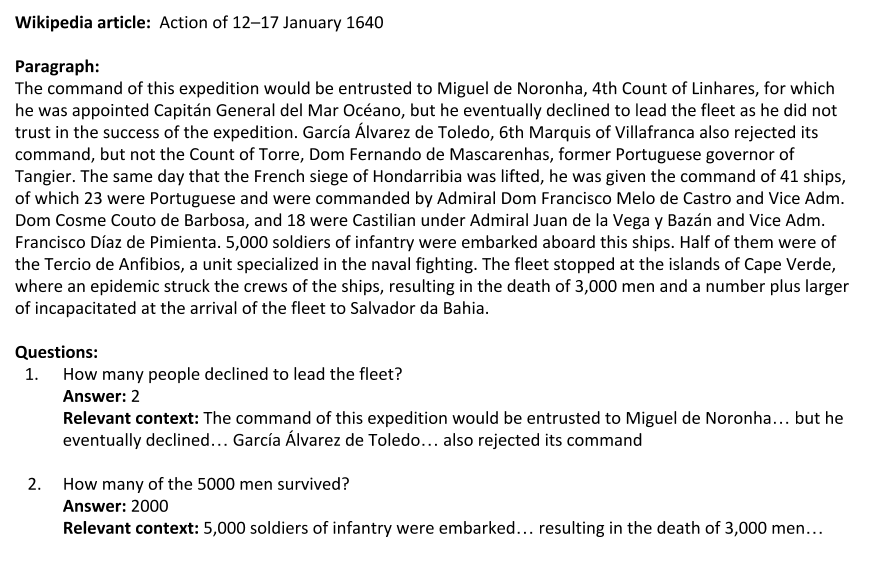
\includegraphics[width=\textwidth]{figures/drop_example.png}
	\caption{A hard reasoning task requiring discrete operations on
unstructured contexts}\label{fig:drop_example}
\end{figure}

Figure~\ref{fig:drop_example} shows an example paragraph along with two
associated questions that resulted from the pilot annotation task. As it can be
seen from the examples, it can seen that the questions at least require identifying entity types (e.g.
\textit{Miguel de Noronha} and \textit{Garcia Alvarez de Toledo} are of type
\textit{people}), solving co-reference over long distances (\textit{3000 men}
refers to a subset of \textit{5000 soldiers}), solving entailment (e.g.
\textit{death} contradicts \textit{survived}). Assuming all this information is
successfully extracted, the questions then require discrete operations (counting
for the first, and difference for the second).

\subsection{Towards building a semantic parser}
To assess the limitations of the techniques presented in this thesis, we applied
the parser we presented in Chapter~\ref{chapter:nlvr} to this task. A
prerequisite for doing so is to first extract relevant information from the
context to make a structure over which the parser can reason.

\paragraph{Information Extraction}
We run a trained open information extraction
(OpenIE) model~\citep{stanovsky2018supervised} over all the sentences in the
paragraph to extract predicate argument structures. This forms the base of our
knowledge graph, which is then augmented as follows: For each argument in each
predicate argument structure, we define additional relations from the text span
to all the numbers and entities (identified by a Named Entity Recognizer) in it.
Given this representation, we directly train a semantic parser using the
procedure described in Chapter~\ref{chapter:nlvr}: We run an exhaustive search
procedure to obtain logical forms for as many questions as possible, and train
an MML parser on it.

\paragraph{Results}
The exhaustive search procedure results in logical forms for only $50\%$ of the
training set, and on a manual inspection of a sample from them, we estimated
that only for $13\%$ of the questions, the search procedure could result in
logical form sets where at least one of the forms was correct. Finally, when the
MML model trained on this dataset had a $7.5\%$ accuracy on the development set.

\paragraph{Challenges}
The biggest hurdle in taking the route of semantic
parsing for this task is the lack of high-quality information extraction. Given that it is
already challenging to extract the kinds of information required by the
questions above, it would be even more difficult to build a semantic parser that
relies on the output of an IE system. One way to deal with this issue is to
train joint models for information extraction over paragraphs, and semantic
parsing over questions. This opens up a new class of NLP tasks where formalism
used for information extraction is determined by the end-task of question
answering.


%\appendix
%\include{appendix}

\backmatter

%\renewcommand{\baselinestretch}{1.0}\normalsize

% By default \bibsection is \chapter*, but we really want this to show
% up in the table of contents and pdf bookmarks.
\renewcommand{\bibsection}{\chapter{\bibname}}
%\newcommand{\bibpreamble}{This text goes between the ``Bibliography''
%  header and the actual list of references}
\bibliographystyle{plainnat}
\bibliography{thesis} %your bib file

\end{document}
